%%%%%%%%%%%%%%%%%%%%%%%%%%%%%%%%%%%%%%%%%
%%            LMU-Vorlage              %%
%%                                     %%
%%         zur Erstellung einer        %%
%%   Dissertation mit pdflatex/latex   %%
%%                                     %%
%%  (2002) Robert Dahlke               %%
%%         & Sigmund Stintzing         %%
%%%%%%%%%%%%%%%%%%%%%%%%%%%%%%%%%%%%%%%%%

\documentclass[12pt]{book}


%%%%%%%%%%%%%%%%%%%%%%%%%%%%
%%   Zusaetzliche Pakete  %%
%%%%%%%%%%%%%%%%%%%%%%%%%%%%

\usepackage{a4wide}
\usepackage{fancyhdr}
\usepackage{graphicx}
\usepackage{german}
\usepackage[bookmarks]{hyperref}
\usepackage[utf8]{inputenc}
\usepackage[style=authoryear]{biblatex}
\bibliography{bibliography}



%%%%%%%%%%%%%%%%%%%%%%%%%%%%%%
%% Definition der Kopfzeile %%
%%%%%%%%%%%%%%%%%%%%%%%%%%%%%%

\pagestyle{fancyplain}
\renewcommand{\chaptermark}[1]%
         {\markboth{\thechapter.\ #1}{}}
\renewcommand{\sectionmark}[1]%
         {\markright{\thesection\ #1}}
\lhead[\fancyplain{}{\bfseries\thepage}]%
    {\fancyplain{}{\bfseries\rightmark}}
\rhead[\fancyplain{}{\bfseries\leftmark}]%
    {\fancyplain{}{\bfseries\thepage}}
\cfoot{}


%%%%%%%%%%%%%%%%%%%%%%%%%%%%%%%%%%%%%%%%%%%%%%%%%%%%%
%%  Definition des Deckblattes und der Titelseite  %%
%%%%%%%%%%%%%%%%%%%%%%%%%%%%%%%%%%%%%%%%%%%%%%%%%%%%%

\newcommand{\LMUTitle}[9]{
  \thispagestyle{empty}
  \vspace*{\stretch{1}}
  {\parindent0cm
   \rule{\linewidth}{.7ex}}
  \begin{flushright}

    \vspace*{\stretch{1}}
    \sffamily\bfseries\Huge
    #1\\
    \vspace*{\stretch{1}}
    \sffamily\bfseries\large
    #2
    \vspace*{\stretch{1}}
  \end{flushright}
  \rule{\linewidth}{.7ex}
  \vspace*{\stretch{5}}
  \begin{center}
    
\includegraphics[width=2in]{FHFLLogo}
  \end{center}
  \vspace*{\stretch{1}}
  \begin{center}\sffamily\LARGE{#5}\end{center}
  \newpage
  \thispagestyle{empty}

  \cleardoublepage
  \thispagestyle{empty}

  \vspace*{\stretch{1}}
  {\parindent0cm
  \rule{\linewidth}{.7ex}}
  \begin{flushright}
    \vspace*{\stretch{1}}
    \sffamily\bfseries\Huge
    #1\\
    \vspace*{\stretch{1}}
    \sffamily\bfseries\large
    #2
    \vspace*{\stretch{1}}
  \end{flushright}
  \rule{\linewidth}{.7ex}

  \vspace*{\stretch{3}}
  \begin{center}
    \Large Bachelorarbeit\\
    \Large an der Fachhochschule Flensburg\\
    \vspace*{\stretch{1}}
    \Large vorgelegt von\\
    \Large #2\\
    \vspace*{\stretch{2}}
    \Large Flensburg, den #6
  \end{center}

  \newpage
  \thispagestyle{empty}

  \vspace*{\stretch{1}}

  \begin{flushleft}
    \large Erstgutachter:  #7 \\[1mm]
    \large Zweitgutachter: #8 \\[1mm]
    \large Tag der m\"undlichen Pr\"ufung: #9\\
  \end{flushleft}

  \cleardoublepage
}




%%%%%%%%%%%%%%%%%%%%%%%%%%%%
%%  Beginn des Dokuments  %%
%%%%%%%%%%%%%%%%%%%%%%%%%%%%

\begin{document}

  \frontmatter


  \LMUTitle
      {Entwicklung eines Microservices zur Augmentierung einer bestehenden monolithischen Anwendung}               % Titel der Arbeit
      {Thomas Peikert}                       % Vor- und Nachname des Autors
      {Berlin}                             % Geburtsort des Autors
      {Angewandte Informatik}                         % Name der Fakultaet
      {Flensburg 2016}                          % Ort und Jahr der Erstellung
      {01.04.2016}                            % Tag der Abgabe
      {Prof. Dr. Milena Zachow}                          % Name des Erstgutachters
      {Prof. Dr. Hans-Werner Lang}                         % Name des Zweitgutachters
      {Pr"ufungsdatum}                         % Datum der muendlichen Pruefung


  \tableofcontents
  \markboth{Inhaltsverzeichnis}{Inhaltsverzeichnis}


  \listoffigures
  \markboth{Abbildungsverzeichnis}{Abbildungsverzeichnis}


  \listoftables
  \markboth{Tabellenverzeichnis}{Tabellenverzeichnis}
  \cleardoublepage


  \markboth{Zusammenfassung}{Zusammenfassung}
  \addcontentsline{toc}{chapter}{\protect Abstract}


\chapter*{Abstract}
Die vorliegende Bachelorarbeit beschäftigt sich mit der Entwicklung von Microservices als Alternative zur ``klassischen'', monolithischen Anwendungsentwicklung. Die integralen Bestandteile von ``Microservice Architektur'', sowie deren Vor- und Nachteile werden erläutert und anhand eines praktischen Beispiels umgesetzt.

Im Rahmen der Arbeit wird ein Microservice entwickelt, der eine bestehende monolithische Betriebsanwendung augmentieren soll. Im momentanen Setup werden Userprofildaten in eine Datenbank geschrieben und aus dieser ausgelesen. Aufgrund der hohen Komplexität dieser Daten und der großen Menge an Daten in der Datenbank, benötigen Profilqueries auf die Datenbank viel Zeit. Da das Auslesen dieser Daten ein integraler Bestandteil der Gesamtanwendung ist, soll hier eine Echtzeit-Schnittstelle bereitgestellt werden. Diese soll in Form einer separaten Anwendung in die bestehende Struktur eingebettet werden.

Hierfür soll ein leseoptimiertes Datenbankformat entwickelt werden, die Anwendung soll eine standardisierte Kommunikationsschnittstelle bieten und kann separat auf einer eigenen Infrastruktur deployt werden. Weiterhin muss eine Anbindung an die bestehende Anwendung geschaffen werden, sodass Änderungen an relevanten Daten in die Queryanwendung gelangen. Dies alles dient dem Zweck, Queries auf Userprofile in soweit zu beschleunigen, dass Anfragen auf Userprofildaten in Echtzeit geschehen können.


  \mainmatter\setcounter{page}{1}
  \chapter{Einleitung}
Wenn Softwaresysteme über Jahre hinweg unkontrolliert wachsen, werden sie oft unübersichtlich und schlecht zu managen. Vor allem, wenn eine junge Firma mehr Wachstum erfährt als erwartet, wird häufig zu wenig Zeit in gute, geordnete Planung von Software gesteckt. Die reine Entwicklung von Features hat dann oft Vorrang. Schnelles Userwachstum führt zu erhöhter Last auf Systemen, Skalierung ist erforderlich. Benutzer fordern neue Features und neue Features bedeuten neuen Code. Schnell kann es passieren, dass die Codebase mehr einem Flickenteppich ähnelt, als einem stabilen Softwaresystem. Für neue Mitarbeiter wird es dann immer schwieriger sich in den bestehenden Code einzuarbeiten. Interdependzen sind kaum mehr absehbar. Auch Deploys gestalten sich in großen Systemen schwieriger. Eine kleine Änderung an einer Stelle im Code erfordert einen redeploy der gesamten Anwendung. Je nach Grad der Automatisierung von Deploys kann dies zur Qual werden. Und selbst wenn Zeit und Arbeit in gute Architektur gesteckt wird, so gehen verschiedene Frameworks doch immer unterschiedlich mit Wachstum um. Interdependenzen im Code führen zu vermischten Strukturen und immer mehr Klassen die zwischen verschiedenen Teilanwendungen geteilt werden. Und oftmals wurde bei einer jungen Firma nunmal nicht die beste Technologie für die Zukunft gewählt, insbesondere weil die Zukunft schlichtweg unklar ist. Der Fokus liegt am Anfang schließlich im Jetzt. Dann heißt es oftmals ``Refactor or Rewrite?''.~\cite[vgl.][]{refactorrewrite}

Die große Herausforderung besteht darin, entweder die bestehende Codebase wieder handhabbar zu machen, um Entwickler- und Betreiberproduktivität wieder zu erhöhen. Oder, idealerweise, ein System gar nicht erst in diesen Zustand kommen zu lassen. In beiden Fällen kann es hilfreich sein, auf den eigenen Architekturstil zu reflektieren.

Eine Architekturweise, die in den letzten Jahren immer mehr an Beliebtheit gewonnen hat, ist die ``Microservice Architektur''. Microservice Architektur verspricht, Code in kleine, gut zu handhabende Systeme aufzusplitten und somit klare Strukturen zu fördern.

In der vorliegenden Arbeit werde ich den Stil der Microservice Architektur vorstellen und die Vor- und Nachteile des Architekturstils benennen. Anhand eines praktischen Beispiels werde ich eine bestehende monolithische Anwendung um einen Microservice erweitern und meine Vorgehensweise erläutern.
Abschließend werde ich Schlüsse zur Umsetzung eines Anwendungsteils mit Microservice Architektur ziehen und das Pattern bewerten.
  \chapter{Microservice Architektur als Weg robuste und skalierbare Anwendungen zu entwickeln}
``Microservice Architektur'' beschreibt einen Stil der Softwareentwicklung, der vor Allem durch die Trennung einer großen Gesamtanwendung, in kleinere, separate Teile gekennzeichnet ist.~\footcite[vgl.][Seite 2]{newman2015building}
Entscheidend für die Microservice Architektur ist im wesentlichen die Abgrenzung zur monolithischen Anwendungsentwicklung, ebenso wie die Abgrenzung zur Service Oriented Architecture.

\section{Microservices als Werkzeug zum Management von Komplexität}
Monolithische Anwendungen bestehen im wesentlichen aus einer einzelnen Einheit.~\footcite[vgl.][]{Fowler:Intro} In einer klassischen drei-Schichten Anwendung (Frontend, Backend, Persistence Layer)~\footcite[vgl.][]{MSDN:TTA}, wie in \autoref{fig:threetier} dargestellt, bietet es sich an, die gesamte Logik in einer Anwendung zu verwalten. Dies ist auch der Standardaufbau der meisten Webframeworks. Es gibt eine Schnittstelle zwischen der clientseitigen und der serverseitigen Anwendung, ebenso wie zwischen der serverseitigen Anwendung und der Datenbank. Unabhängig wie unübersichtlich ein System mit zunehmender Größe wird, das zusammenhalten dieser Anwendungsteile ist der default Weg. Schwer zu handhabende, komplexe und große monolithische Anwendungen entstehen häufig dann, wenn bei Wachstum mit der Zeit dieser Aufbau nicht überdacht wird.~\footcite[vgl.][]{infaktuell}
\begin{figure}[!ht]
    \caption{Drei-Schichten Anwendungsverteilung (\cite{ThreeTieredDistribution})}
    \label{fig:threetier}
    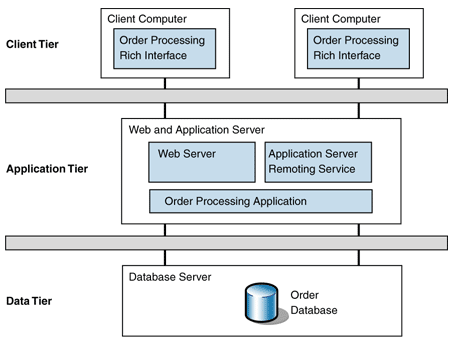
\includegraphics[width=\textwidth]{three_tier_application}
\end{figure}

Anstatt einer großen Anwendung, deren einzelne Teile gemeinsam deployt werden, in einem gemeinsamen repository liegen und auf der Ebene der genutzten Programmiersprache kommunizieren, wird bei der Microservice Architektur die Gesamtanwendung hingegen in einzelne Teilanwendungen aufgesplittet. Diese liegen in separaten Repositories, können getrennt voneinander deployt werden und kommunizieren über externe Schnittstellen. Diese separaten Teilanwendungen sind meist anhand von Aufgabengebieten getrennt und identifiziert. Die Trennung nach Single Responsibility Principle~\footcite[vgl.][Seite 108]{Martin:SRP} wird hier von der Ebene des Codes in die Ebene der Gesamtarchitektur gehoben.

Ein Architekturstil, der der Microservice Architektur ähnelt, ist die ``Service-Oriented Architecture''. Aufgrund der ähnlichen Ansätze, die dieser Architekturstil verfolgt, sollte er näher betrachtet werden.
Service-Oriented Architecture (SOA) hat sich ebenfalls entwickelt, um die Probleme großer, monolithischer Anwendungen zu lösen.~\footcite[][Seite 8]{newman2015building} Mit Hilfe von Services, soll wiederverwendbarer Code geschaffen werden, der dann von verschiedenen Endanwendungen genutzt werden kann. Die Kommunikation findet über Netwerke statt und nicht mehr über direkte Aufrufe im Code. Auch SOA soll es einfacher machen Code zu organisieren, zu strukturieren und bei Bedarf zu ersetzen. Warum entsteht nun also der Trend der Microservices, wenn SOA einen ähnlichen Ansatz verfolgt? Ein großes Problem von SOA liegt eigentlich in den damit verbundenen Technologien wie SOAP, vendor middleware und der nicht ausreichend klaren Trennung der Services.~\footcite[][Seite 8]{newman2015building} 
Ein weiterer Unterschied zwischen SOA und Microservice Architektur ist grundsätzlich auch die Kommunikation zwischen den Services. Wo SOA häufig zu komplexer Logik mit dem Enterprise Service Bus\footcite[][]{esb} tendiert, setzt die Microservice Architektur Gemeinschaft gemeinhin auf das an das Unix Prinzip der ''Pipes and Filters''\footcite[vgl.][]{microsoft:pipes} angelehnte Prinzip der ''Smart Endpoints und Dumb Pipes''.~\footcite[vgl.][]{Fowler:Intro}
Weiterhin teilen sich SOA Services häufig Datenbanken, in der Welt der Microservices ist dies hingegen nicht verbreitet. SOA scheint zudem nicht klar genug definiert zu sein.~\footcite[vgl.][]{Fowler:Intro} Daher ist es ratsam einen klarer definierten Begriff, wie den der Microserice Architektur anzustreben.~\footcite[][]{Fowler:Intro}

Die Aufteilung einer monolithischen Gesamtanwendung in kleinere Services ist jedoch keineswegs ein Allheilmittel für alle Probleme. Microservice Architektur birgt seine ganz eigenen Herausforderungen. Microservice Architektur bringt demnach vor allem Unterschiede mit sich. Die Frage ob sich diese positiv oder negativ auswirken, hängt ganz individuell von der bestehenden Anwendung, dem Entwicklerteam und den vorhandenen Resourcen ab.

\section{Herausforderungen und Potentiale von Microservices}
Wie jeder Architekturstil bieten auch Microservices zwar ihre Vorzüge, kommen aber auch immer mit ganz eigenen Kosten.~\footcite[vgl.][]{Fowler:Guide}
Bei der Entscheidung ob Microservices im Unternehmen eingesetzt werden sollten, müssen diese Vor- und Nachteile der Microservice Architektur abgewogen werden.
Im folgenden werde ich die Vor- und Nachteile des Architekturstils auf den verschiedenen Ebenen der Struktur des Codes, Technologieheterogenität, Systemverteilung, Testing, Deployment, Skalierbarkeit und Entwicklungszeit erläutern.

\subsection{Struktur des Codes}
Microservice Architektur verspricht zum einen klarere Strukturen. Seperate, nach Aufgabengebiet unterteilte Services führen zu klar strukturierten Codebases. Diese aufgeteilten Codebases verschaffen einen besseren Überblick, sodass sich Entwickler leichter in ein Aufgabe einarbeiten können ohne sich durch irrelevante Codeteile arbeiten zu müssen. Gerade in größeren Teams ist dies von großem Vorteil. Je mehr parallel an voneinander abhängigen Codeteilen gearbeitet wird, desto mehr merge Konflikte entstehen. Auch wenn die eigentlichen Aufgaben komplett voneinander getrennt sind, kommt es häufig zu Konflikten. Je vermischter der Code ist, desto mehr Konflitke enstehen. Ähnlich wie das Single Responsibility Principle auf Methoden- oder Klassenebene gilt, so kann man es auch auf Service Ebene als geltend ansehen. Getrennte, klar strukturierte Codeteile erhöhen die Wiederverwendbarkeit, erleichtern die Einarbeitung und das Management des Codes. Ebenso können Änderungen leichter eingearbeitet werden, da die Chance von Seiteneffekten reduziert ist. Komplexitäten werden demnach nicht per sé reduziert, sie werden jedoch aufgetrennt und verschoben. Somit werden sie leichter zu handhaben.

So lassen sich zum Einen kleinere, autonome Anwendungsteile aus Entwicklersicht besser verwalten. Die einzelnen Anwendungsteile müssen jedoch über eine externe Schnittstelle kommunizieren. Diese Aufrufe, die in der Regel über das Intra- oder Internet stattfinden sind aufwändiger als simple Code Calls. Wie diese API calls stattfinden ist nicht zwangsläufig vorgeschrieben [WAS FUR MOGLICHKEITEN GIBT ES]. Im Allgemeinen gilt jedoch: Verteilte Systeme sind schwieriger zu programmieren, da remote calls langsam und fehleranfälliger sind.~\footcite[vgl.][]{Fowler:Guide}

\subsection{Technologieheterogenität}
Separate Services ermöglichen auch, komplett verschiedene (FIX DIVERSE?) Technologiestacks einzusetzen. Im Gegensatz zur Erweiterung einer monolithischen Anwendung, muss hier theoretisch nur bedingt auf die bereits eingesetzten Technologien geachtet werden. Ein separater Service mit separater Datenbank kann durchaus eine andere Datenbanktechnologie verwenden. Da über den separaten Service ohnehin ein separates Datenbankadapter implementiert werden muss, ist es aus reiner Implementierungssicht nicht nachteilig eine andere Datenbanktechnologie zu wählen. Hierbei kann durchaus auf die für den Anwendungsfall spezifischen Optimierungsmöglichkeiten geachtet werden. Ebenso kann eine für den Anwendungsfall optimierte Programmiersprache gewählt werden.
Das diese diverse (FIX ENGLISCH DIVERSE) Technologiewahl aus technischer Sicht möglich und ratsam ist, heißt jedoch keineswegs, dass sie tatsächlich so gewählt werden sollte. Die bestehenden Technologien in einem Unternehmen, welches beschließt eine große, bestehende Anwendung in Microservices aufzuteilen oder um einen Microservice zu erweitern, sind in der Regel tried and tested. Eine Vielzahl der Entwickler des Unternehmens wird mit den bestehenden Technologien vertraut sein. Fällt ein Entwickler aus, sind vermutlich noch genug andere Entwickler mit ähnlichen Fähigkeiten vorhanden um in dringenden Fällen die Arbeit zu übernehmen. Wählt man nun aber eine neue Programmiersprache, eine neue Datenbanktechnologie und neue Monitoring Tools aus, so ist dies ggf. nicht nur mit erhöhter Einarbeitungszeit verbunden, sondern auch mit höheren Managementkosten. Müssen neu eingstellte Entwickler nun den gesamten Technologiestack beherrschen oder nur einen der zwei Teile? Sind immer ausreichend Entwickler vorhanden um einen ausfallenden Entwickler zu kompensieren? Was passiert wenn der Entwickler des neuen Go Microservices kündigt und kein anderer Entwickler Go beherrscht? Die technologische Heterogenität kommt demnach zu einem Preis. Man sollte genau abwägen, bis zu welchem Grad die Diversifizierung des Technologiestacks lohnenswert ist.~\footcite[vgl.][Seiten 5, 6]{newman2015building}
Die Definition eines klaren, ``erforderten Standards''~\footcite[vgl.][Seiten 20, 21]{newman2015building} bietet sich hierzu an. Twitter und Netflix limitieren hierzu z.B. auf Technologien die unter der Java Virtual Machine (JVM) laufen (FIX FORMULIERUNG).~\footcite[][Seite 6]{newman2015building} Entwickler können so eine neue Programmiersprache wie Scala oder JRuby wählen, es wird jedoch auf bekannte Technologien im Betrieb des Servers gesetzt. Dieser erforderte Standard bezieht sich auch auf die gewählten Wekzeuge zum Monitoring und die eingesetzten Schnittstellentechnologien.~\footcite[vgl.][Seite 21]{newman2015building} So sollte nicht jeder Microservice ein anderes Montoring Tool verwenden und die Clientanwendung nicht zu jedem Microservice eine andere Schnittstellentechnologie einbinden.

\subsection{Verteilte Systeme}
Eine große Herausforderung bei der Verwendung von Microservice Architektur, ist vor allem auch die Tatsache das es sich schlichtweg um verteilte Systeme handelt.~\footcite[][]{microtradeoffs}
Tanenbaum und Van Steen definieren Verteilte Systeme als Sammlung unabhängiger Computer, die zum Benutzer als eine einzige, kohärente Einheit erscheinen.~\footcite[][Seite 2]{tanenbaum2002distributed}
Zwar haben wir klar getrennte Systeme, die von der Codebase her gut zu managen sind, remote calls sind aber immer fehlerbehaftet. Der Service kann über das Netzwerk unnerreichbar sein, die Antwort zu lange dauern und zu einem Timeout führen und dauern im Allgemeinen länger als code calls. Timeouts und langsame Serviceantworten können natürlich über asynchrone Aufrufe umgangen werden, aber asynchrone Aufrufe bringen ihre eigenen Probleme mit sich. Nicht umsonst spricht man hier oft in der Entwicklung von der Callback-Hell.~\footcite[vgl.][]{callbackhell} Zweifelsohne kann man Die Callback-Hell vermeiden, die Integration einer Netzwerkschnittstelle in die Codebase birgt aber immer Gefahren. Man kann schlichtweg nicht von einem sicheren Netztwerk ausgehen, demnach bedarf es einem Sicherheitsmechanismus zur Authentifizierung. Bandbreite kann ggf. mit Kosten verbunden sein und ist nicht unbegrenzt verfügbar und das Netztwerk kann unzuverlässig sein.~\footcite[vgl.][]{distributedfallacies}

Zudem müssen separate Systeme auch einzeln überwacht werden. Wo monolithische Anwendungen eine Quelle von Metriken, eine Anwendung zu überwachen und eine Anwendung zu deployen haben, haben Microservices viele.~\footcite[vgl.][]{Heroku:GoMicro}

\subsection{Testing}
\label{section:testing}
In diesem Zug sollte auch das Thema Testing angesprochen werden. Testen, gerade über die Grenzen von Services hinweg, ist durchaus eine Herausforderung die es zu meistern gilt (FIX FORMULIERUNG). Auf der anderen Seite tendieren große monolitische Anwendungen dazu, eine lange Testlaufzeit zu haben. Ab einer gewissen Größe ist es kaum noch möglich, dass der Entwickler alle Tests lokal ausführt. Der Einsatz von Continuous Integration schafft hier natürlich Abhilfe, doch auch hier sind die Ressourcen nicht unbegrenzt. Bei einer Vielzahl von Entwicklern, die parallel arbeiten, können auch mit mehreren concurrent builds Buildstaus oft nicht vermieden werden. Separate Codebases mit separaten kleineren Tests, haben hier vor Allem den großen Vorteil, dass nicht alle Tests immer erneut ausgeführt werden müssen.

Somit verhält sich die Gesamttestlaufzeit t stark unterschiedlich. Die Parallelität des Continuous Integration Servers vernachlässigend, berechnet sich die Gesamtlaufzeit der Tests wie folgt:

\begin{center}
$ t = \displaystyle\sum_{i=1}^{n} t_i $
\end{center}

\noindent wobei n die Anzahl der parallel arbeitenden Entwickler und $t_i$ die Testlaufzeit der bearbeiteten Codebase ist.

Die Gesamttestlaufzeit berechnet sich demnach additiv aus den Einzeltestlaufzeiten der jeweiligen Codebases. Da die Einzeltestlaufzeit bei Microserices wesentlich geringer ist, kann hier enorm an Zeit gespart werden.

Bei vier Entwicklern und einer monolithischen Testlaufzeit von zehn Minuten erreicht man eine Gesamttestdauer von 40 Minuten

\begin{center}
$ t = \displaystyle\sum_{i=1}^{4} t_i = 10m + 10m + 10m + 10m = 40m $
\end{center}

\noindent Bei identischer Codebase, beliebig verteilt auf vier Microservices mit identischer Gesamttestdauer von zehn Minuten, erreicht man jedoch nur eine Testdauer von zehn Minuten 

\begin{center}
$ t = \displaystyle\sum_{i=1}^{4} t_i = 3m + 4m + 1m + 2m = 10m $
\end{center}

\noindent Natürlich muss man zu der reinen Testdauer der Codebase einen gewissen Overhead im CI System einplanen, der nicht proportional zur Testdauer ist, dieser ist aber für die Ergebnisse zu vernachlässigen. Ebenso sollte die Zahl von Testfällen bei Microservice Architektur etwas erhöht sein, aber auch dies sollte im Vergleich zu einer großen monolithischen Anwendung noch zu einer großen Ersparnis führen.

Eine große Herausforderung beim Einsatz von Microservices ist jedoch das Testen selbst. Treten im Live Betrieb Fehler auf, ist es nicht leicht herauszufinden wo der Fehler wirklich entsteht. Ist es ein Fehler im konsumierten Service, im konsumierenden Service oder in der Kommunikation zwischen den beiden Seiten?

\begin{wrapfigure}{l}{0.5\textwidth}
    \caption{Das Testing Board zum Testen mit Microservices (\cite{rails:soa})}
    \label{fig:testboard}
    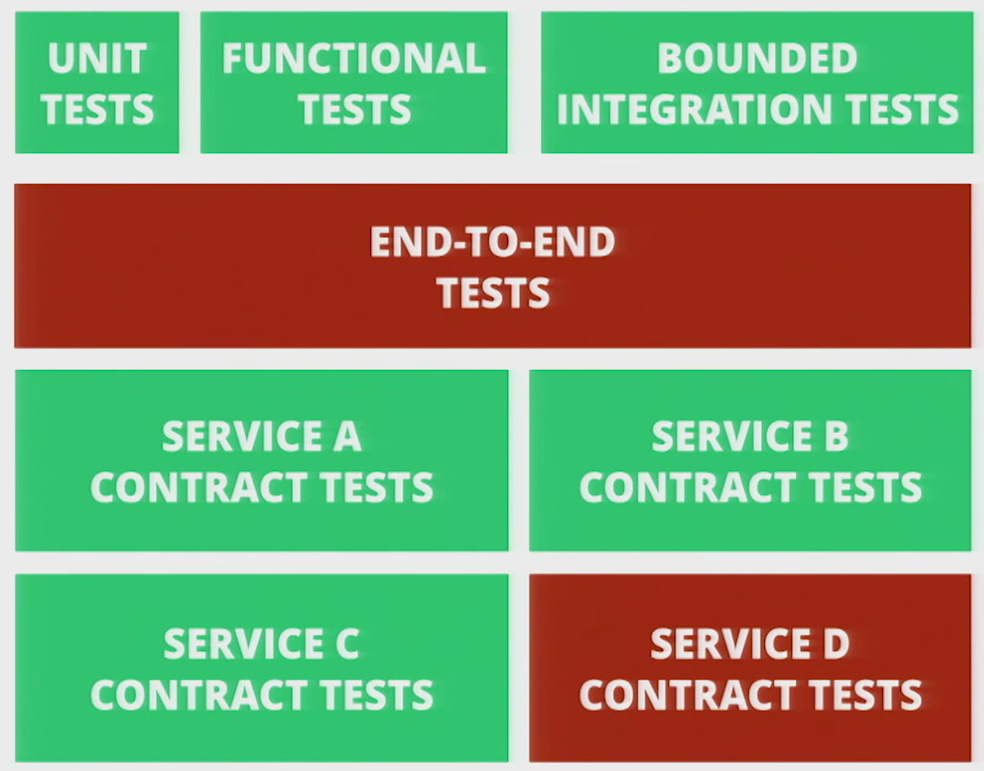
\includegraphics[width=0.5\textwidth]{testing_board}
\end{wrapfigure}

Hierzu bietet es sich an verschiedene Testebenen einzuführen. Zum Einen sollten natürlich immer sowohl der Client, als auch der Server selbst voll getestet sein. Als Weiterführung dessen, bieten sich sogenannte ``Bounded Integration Tests''\footcite[vgl.][]{rails:soa} an. Bounded Integration Tests mocken im Endeffekt konsumierte Services. Dies kann zum Einen in-process geschehen, zum Anderen out-of-process. Beim in-service mocken wird quasi vorgegeben man würde mit einem externen Service sprechen. Wir erwarten also, dass der Service auf eine bestimmte Anfrage in einer bestimmten Weise antwortet und mocken es entsprechend. Beim out-of-process Mocking erstellen wir einen Pseudoservice der weiß wie er auf bestimmte Services zu antworten hat. Hier wird also der Service selbst gemockt. (FIX SCHLECHT FORMULIERT)
Als Erweiterung der Bounded Integration Tests, die den eigenen Service und die abgeschickten Abfragen testet, bieten sich Contract Tests an.~\footcite[vgl.][]{fowler:contracts} Contract Tests testen den konsumierten Service, indem Sie Anfragen verschicken und die zurückgelieferten Antworten überprüfen. Hier testen wir also quasi den Bounded Context des konsumierten Services und die Kommunikation mit ihm. Außerdem überprüfen wir hier aber auch unser Verständnis vom Service, es muss schließlich nicht zwangsläufig der Service fehlerhaft sein, es kann auch unser Verständnis des Services oder schlichtweg dessen Dokumentation fehlerhaft sein.
Bounded Integration Tests und Contract Tests, ergänzt durch end-to-end Tests bilden mit den üblichen Unit und Integration Tests der Einzelanwendungen einen guten Test Stack, der die Fehlerfindung erheblich erleichtert. So würde ein einfacher Fehler im Betrieb der in \autoref{fig:testboard} dargestellten Anwendung ohne diese komplexen Tests schwer nachzuvollziehen sein. Mit Hilfe des Einsatzes aller Tests auf dem Test Board, kann die genaue Fehlerquelle jedoch leicht identifiziert werden.

Interessant sind hier auch Ansätze wie ``Failure Injection Testing''.\footcite[][]{netflix:fit} Hier werden Systemfehler bewusst und kontrolliert auf kleiner Skala provoziert und dann das Verhalten des Gesamtsystems beobachtet. Konkret ist hier z.B. Netflix's\footnote{http://www.netflix.com/} Chaos Monkey\footcite[][]{netflix:chaosmonkey} zu nennen. Alle Dienste von Netflix werden auf Amazon Web Storage (AWS)\footnote{https://aws.amazon.com/} betrieben. AWS Bietet hier Auto Scaling Groups (ASG). Je nach Last werden neue Serverinstanzen innerhalb festgelegter Regeln hochgefahren um die Last auf den Services angemessen zu handhaben. Der Chaos Monkey fährt nun auf einer bestimmten ASG randomisiert Instanzen herunter. Nach den Regeln der ASG sollte nun eine neue Instanz hochgefahren werden um die Alte zu ersetzen. Das System sollte nun eine messbare, aber keine relevante Verschlechterung der Antwortzeiten des Services erfahren. Interessant ist hier, wie gut das System mit dem Ausfall umgeht, wie schnell das System wieder die volle Leistung hat (mean time to recovery) und ob ggf. durch das Zusammenspiel von Services größere Fehler zustande kommen als erwartet. Aufgrund des kleinen, kontrollierten Ausfalls, ist die Wahrscheinlichkeit allzu großer Auswirkungen, selbst bei unerwarteten Fehlern, gering. Die Erkenntnisse des Failure Injection Testings können jedoch wertvoll sein und größere Probleme bei umfangreicheren Ausfällen vermeiden. Netflix selbst bewertet diese Testmethode als vollen Erfolg und weitete Failure Injection Testing vom Chaos Monkey auf weitere Testgebiete aus. So finden sich heute fünf weitere Monkeys und der Chaos Gorilla im aktiven Einsatz.\footcite[][]{netflix:army}.

Ein weiterer Ansatz, der unter das Testen im Produktionsbetrieb fällt, sind graduelle bzw. staged Rollouts. Hier wird eine neuer Dienst nur für einen bestimmten Teil der Anfragen freigeschaltet. In der Regel wird hier einfach mit Hilfe eines dem Load Balancing ähnlichen Systems prozentual immer mehr der Anfragen auf den neuen Dienst geleitet. Gleichzeitig wird die Rate und die Art der auftretenden Fehler beobachtet. Steigt die Fehlerrate mit zunehmender Umleitung der Anfragen oder treten neue Fehler auf, kann dies in der Regel auf den neuen Dienst zurückgeführt werden. Ein ähnliches System nutzt Google zum Beispiel beim Veröffentlichen neuer Android Versionen.\footcite[vgl.][]{Google:staged}

All diese Ansätze ersetzen natürlich keineswegs das klassische Testen vor der Veröffentlichung von Software. Sie bieten sich aber als ergänzende Testmethoden an um vor Allem die wachsende Komplexität von Softwaresystemen zu testen.

\subsection{Deployment}
Die Aufteilung einer einzelnen Codebase, die zusammen deployt wird, in mehrere Codebases bringt zwingend ebenfalls Änderungen mit sich.
Zum Einen können relativ kleine Änderungen leichter deployt werden, da nicht das gesamte System erneut deployt werden muss. Bei großen, komplexen Anwendungen können diese großen deploys ein nicht zu vernachlässigendes Risiko bilden. Und ist das Deployment einer Anwendung risikoreich, wird im Allgemeinen seltener deployt. Features werden erst später deployt, doch mit wachsenden Unterschieden zwischen Deployments, wächst auch das Risiko von Fehlern.~\footcite[vgl.][Seite 6]{newman2015building}
Separate Deploys von Microservices machen die Versionierung von diesen jedoch um so wichtiger~\footcite[vgl.][Seite 62]{newman2015building}~\footcite[vgl.][]{Vergleichsartikel}. Breaking Changes können nicht einfach deployt werden und da gleichzeitige Deploys verschiedener, mit einander kommunizierender Services nicht möglich sind, müssen diese Deploys schrittweise und kontrolliert durchgeführt werden: Zunächst muss der Service um eine neue Version erweitert werden, die alte Schnittstelle darf hierbei nicht verändert werden. Meist werden hierzu API Versionen genutzt. So kann die erste Schnittstelle über die URL

\begin{lstlisting}[language=Ruby]
https://meinservice.tld/api/v1/eineRoute
\end{lstlisting}

\noindent angesprochen werden. Diese Schnittstelle wird von den Änderungen nicht tangiert. Die neue Schnittstelle umfasst sowohl die neuen, als auch alle alten, weiterhin gewünschten, Funktionen. Sie ist über die URL

\begin{lstlisting}[language=Ruby]
https://meinservice.tld/api/v2/eineRoute
\end{lstlisting}

\noindent anzusprechen. Nach Deploy dieser neuen Service Version, wird als nächstes der konsumierende Code geupdated. Hierbei wird die Nutzung der Funktionen auf die neue Version aktualisiert und die Request auf die neue URL umgeleitet. Alle Referenzen zur alten Route des konsumierten Services sollten hierbei entfernt werden. Abschließend kann, solange sichergestellt ist, dass die alte Service Version nicht mehr genutzt wird, der Service ein weiteres mal geupdated werden. Hierbei wird der Code der alten Version entfernt. Dies ist in der Regel nur bei firmeninternen APIs üblich. Externe APIs sollten in veralteten Versionen noch eine gewisse Zeit angeboten werden. Sollte in der neuen API Version ein Fehler auftreten, muss, vorausgesetzt v1 ist unverändert zu erreichen, nur der konsumierende Service gerollbacked werden.
Datenbankmigrationen müssen hier nach dem gleichen Prinzip ebenso in mehreren Schritten durchgeführt werden.
Versionierung ist vor Allem bei APIs mit externen Konsumenten, wie Clientanwendungen, da Updates hier nicht sofot geschehen und nicht kontrolliert werden kann, ob noch alte Routen aufgerufen werden. Bei reinen browserseitigen Clientanwendungen Anwendungen ist die Versionierung nicht zwingend notwendig, kann aber dennoch nützlich sein.
Das deployment kann also in vielen Fällen bei Microservices leichter sein, gestaltet sich bei großen Änderungen jedoch schwieriger.

\subsection{Skalierbarkeit}
Ein weiterer interessanter Punkt zum Betrieb von Microservices, ist das Thema der Skalierbarkeit.
Das ``Scale Cube''\footcite[][]{abbott2009art} Modell beschreibt die drei Dimensionsen der Anwendungsskalierbarkeit. Klassische Anwendungsskalierung geschieht vor allem auf der X-Achse, der horizontalen Duplikation\footcite[][]{abbott2009art}. Skaliert wird hier, indem eine Anwendung dupliziert wird. Ein Load Balancer verteilt dann, nach bestimmten Regeln, die ankommenden Requests auf verschiedene Server.~\footcite[vgl.][]{loadbalancing} 

\begin{figure}[!ht]
    \caption{Die Dimension des Skalierens (\cite{abbott2009art})}
    \label{fig:scalecube}
    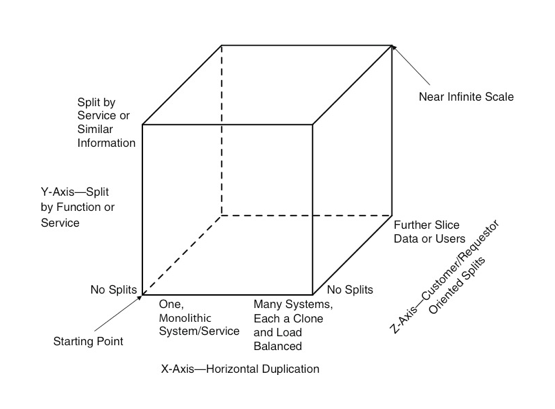
\includegraphics[width=\textwidth]{scale_cube}
\end{figure}

Die Skalierung monolithischer Anwendungen beschränkt sich in der Regel insbesondere auf dieses Load Balancing.~\footcite[vgl.][]{infaktuell} 
Da die Anwendungsreplikationen funktional identisch sind, ist die verteilte Last unabhängig von den einzelnen Anwendungsteilen. Diese können eine unterschiedliche Individuallast haben, dies kann jedoch über den Load Balancer nicht beachtet werden.

Bei Microservices kann nun weiterhin auf der Y-Achse skaliert werden. Hier handelt es sich um eine funktionale Dekomposition\footcite[][]{abbott2009art}. Anwendungen werden hier in verschiedene Services unterteilt. Jeder Service ist für eine bestimmte Funktion zuständig. So kann weitaus granulärer skaliert werden. erhält ein Teilsystem besonders viel Last, kann dieses beliebig skaliert werden. Die anderen Teilsysteme bleiben davon unberührt. Dies optimiert sowohl Leistung, als auch Kosten.

Zusätzlich können sowohl monolithische Anwendungen, als auch Microservice auf der Z-Achse skaliert werden. Hier handelt es sich vor Allem um Datenpartionierung. So werden Datenbanksysteme oft gesharded.\footcite[][]{microsoft:sharding} Dieses Sharding trennt Daten die eigentlich zusammengehören. Anhand bestimmter Kriterien werden Rows einer Datenbank auf verschiedene Systeme verteilt. Diese Partitionen Bilden sogenannte Shards und können z.B. auf verschiedene Datenabankserver verteilt werden.

\subsection{Entwicklungszeit}
Zu guter Letzt sollte man die reine Entwicklungszeit betrachten. Zwar ist die separate Codebase im Nachhinein ggf. leichter zu verwalten, die initiale Entwicklung ist aber durchaus mit einem gewissen Mehraufwand verbunden. Die Wahl der optimalen Technologien ist mit Recherche verbunden, der Einsatz neue Technologien darüber hinaus mit einer Einarbeitungszeit. Das initiale Setup von Programmiersprache, Framework und Datenbank ist ein zusätzlicher Aufwand, der bei der Erweiterung einer bestehenden Codebase nicht anfällt. Hinzu kommt außerdem die Einrichtung des Deployments. Git, Continuous Integration / Deployment, Servereinrichtung, sowie das Monitoren und Warten der Server sind vor allem zum Beginn des Lebenszyklus eines neuen Microservices ein nicht unerheblicher Mehraufwand. Dies und andere Herausforderungen gegen die Potentiale der Microservice Architektur abzuwägen, muss im konkreten Einzelfall immer individuell geschehen.

\section{Der Weg zum Microservice}
Wenn in einem Unternehmen entschieden wird, Microservice Architektur einzusetzen, stellt sich die Frage, wie dies konkret umgesetzt wird. Eine monolithische Anwendung kann um Microservices ergänzt werden oder umgearbeitet werden um die monolithische Struktur auf Microservices umzustellen.
Man kann demnach in verschiedene Ausganssituationen unterscheiden:
\begin{description}
  \item[Aufsplittung] \hfill \\
  Ein bereits bestehender Anwendungsteil soll zu einem Microservice umgebaut werden. Der bestehende Code soll nicht ersetzt, sondern lediglich verschoben werden. Die Schnittstellen zum bestehenden Code müssen erneuert werden.
  \item[Rewrite] \hfill \\
  Ein bereits bestehender Anwendungsteil soll von Grund auf neu geschrieben werden. Bestehender Code wird ersetzt und der neue Code als separater Service in die bestehende Anwendung integriert.
  \item[Erweiterung] \hfill \\
  Ein neuer Anwendungsteil soll entwickelt werden. Die Aufgaben des neuen Anwendungsteils sind weder in der bestehenden Anwendung, noch extern vorhanden. Es wird neuer Code geschrieben und in die bestehende Anwendung integriert.
\end{description}
Zwar unterscheiden sich die drei aufgeführten Ausgangssituationen im Endprodukt nicht zwangsläufig, in der Entwicklung des Microservices muss aber grundlegend anders vorgegangen werden. 

Der erste und zweite Fall unterscheiden sich nicht grundlegend. Die bestehende Schnittstelle zur betroffenen Funktion muss komplett überarbeitet werden. Sowohl in der bestehenden, als auch in der neu entstehenden Anwendung muss diese Schnittstelle geschaffen werden. Auch wenn nur existierender Code verschoben wird, muss eine komplett neue Schnittstelle geschaffen werden. Wo vorher code calls genutzt wurden, werden nun API calls genutzt.
Welches dieser zwei Vorgehensweisen mit mehr Aufwand verbunden ist, hängt zum Großteil von der Komplexität und Struktur der bestehenden Anwendung ab. Auch wie modular der bereits existierende Code ist, ist entscheidend. Je nach Alter des bestehenden Codes ist eine Neuentwicklung teils ratsam. Da die Umarbeitung ohnehin mit erheblichem Arbeitsaufwand verbunden ist, bietet sich eine Optimierung des bestehenden Codes häufig an. Bei großen, komplexen Legacy Anwendungen ist dies in der Praxis aber häufig nicht ratsam.
Bei der Aufsplittung des Monolithen bietet es sich hierbei an, sich am Saum (engl. seams ~\footcite[vgl.][Seite 29 ff.]{feathers2004working}) orientiert werden. Codeteile, die isoliert sind und ohne Seiteneffekte geändert werden können, eignen sich besonders gut um in separate Services verschoben zu werden. Natürlich ist es alles eine Frage der konkreten Problematik, ob ein Service frei, neu gewählt werden kann oder aus Notwendigkeit, unabhängig vom Grad der Komplexität, geschaffen werden muss.

Im dritten Fall kann der neue Anwendungsteil nach idealen und neuen Vorstellungen entwickelt werden. Zwar muss auch hier eine Integration zum bestehenden Code geschaffen werden, es gibt aber keine bisherige Implementation die beachtet werden muss. Die Entwickler haben die freie Wahl, die bestmögliche Integrationsform zu wählen. Dies kann häufig zum besten Endprodukt führen, da keine Einschränkungen durch bestehenden Legacy Code die Programmierung beeinträchtigen. Natürlich wird hier aber ein komplett neues Feature entwickelt. Die Konzeption der Architektur, des Codes und die komplett neue Entwicklung können hier mit einem wesentlichen Mehraufwand verbunden sein. Die Integration in die bestehende Anwendung sollte aber in der Regel mit weniger Problemen verbunden sein.

Weiterhin stellt sich die Frage wie der Microservice in Betrieb genommen wird. Bildet der Microservice ein neues Feature, kann er schlicht eingebunden werden. Ersetzt der neue Service jedoch einen bestehenden Anwendungsteil, sollte hier mitunter nicht sofort die Anwendung umgestellt werden. Wie in \autoref{section:testing} beschrieben, bietet es sich an hier nach einem dem Load Balancing ähnlichen System nach und nach mehr Last auf den neuen Anwendungsteil zu leiten und das Fehlerverhalten zu überwachen.
Ein Ansatz zum allgemeinen Ersetzen alten Codes durch neuen, ist das Strangler Pattern.~\footcite[][]{Fowler:Strangler} An geeigneten Stellen wird hier im Live Betrieb immer mehr Code an sich eignenden Stellen ersetzt und parallel betrieben. Eine neue Anwendung kann hier in agiler Weise um den bestehenden Code gewoben werden und diesen Schlussendlich komplett ersetzen.
%(FIX Strangler Pattern hier nur angerissen, Dopplung. hmmm)
  \chapter{Entwicklung einer real-time Query Anwendung zur Beschleunigung von Userprofilqueries}
In der bestehenden Betriebsanwendung werden Nutzer zum Zweck von Umfrageteilnahmen verwaltet. Nutzer pflegen Profilangaben, um dann passgenau zu Umfragen eingeladen zu werden.
Ein wesentlicher Bestandteil der Anwendung bildet das Abfragen eben dieser Nutzerprofildaten. Um für Umfragen passgenau Teilnehmer auszuwählen, gibt es in der Profildatenbank, die knapp 400.000 Nutzer umfasst, 176 Profilfelder. Diese können in allen denkbaren Kombinationen abgefragt werden. Die besteheden Datenbankabfragen geschehen aufgrund ihrer langen Laufzeit asynchron. Hier soll eine neue Echtzeitschnittstelle geschaffen werden.

\section{Real-time Anforderungen erzwingen eine neue Entwicklung}
Da das Finden von Umfrageteilnehmern und demnach das Abfragen der Profilfelder einen wesentlichen Kern der Betriebsanwendung bildet, besteht dieser Teil der Anwendung mit am längsten. In den fast 3 1/2 Jahren ist sowohl die Anzahl der Nutzer, also auch die Anzahl der Profilfelder enorm gewachsen, weitaus mehr als initial erwartet. Im Laufe der Zeit stellte sich heraus, das die gewählte Datenbanktechnologie MongoDB, die gewählte Datenstruktur und die Art wie gequeried wird, nicht optimal und daher nicht schnell genug sind. Da das Abfragen der Profilfelder wesentlichster Bestandteil des Kerngeschäfts ist und die Defizite die Situation mit wachsender Nutzer- und Kundenzahl nur verschärfen, wurde deutlich, dass eine Überarbeitung der bestehenden Strukturen notwendig ist.

Das Ziel der Neuentwicklung ist vor Allem, die Profilqueries zu beschleunigen, ohne dadurch an anderen Stellen Performance einzubüßen. Da viele Queries, besonders auf solche Felder, die nicht durch einen Index abgedeckt sind, sehr langsam sind, soll hier eine signifikante Zeitersparnis erreicht werden. Zum Anderen soll aber gleichzeitig auch die Struktur des Codes verbessert werden. Fast die gesamte Anwendung befindet sich zur Zeit in einem Repository. Die Strukturen sind zum Teil sehr vermischt und Abhänigkeiten bestehen auch dort, wo keine bestehen sollten. Der neu entworfene Code soll klare Strukturen und klare Schnittstellen besitzen.

\section{Majestic Monolith vs Minimal Microservice}
Um die genannten Probleme zu lösen, können jedoch verschiedene Lösungsansätze zur Optimierung verfolgt werden. Zum Einen kann eine neue Datenbanktechnologie mit optimiertem Schema gewählt werden. Zum Anderen kann der Code auf Geschwindigkeit optimiert oder komplett neu geschrieben werden.
Da die in der Anwendung eingesetzte Datenbank MongoDB noch für weitere Teile der Anwendung genutzt wird, kann sie nicht komplett ausgetauscht werden. Da es sich jedoch zur Optimierung sowohl anbietet eine neue Datenbanktechnologie einzusetzen, als auch den Code zu verbessern, bietet sich die Entwicklung eines separaten Microservices an. Hier kann eine optimierte Datenbanktechnologie eingesetzt werden ohne die bestehende Anwendung um weitere Strukturen und somit Komplexitäten zu ergänzen. Der Code kann restrukturiert und verbessert werden, in dem klarere und eindeutigere Strukturen und Aufteilungen geschaffen werden

Des Weiteren erlaubt es ein separater Service passgenauere Skalierung. Durch dynamisches Hosting kann so also nicht nur die inhärente Performance von Code und Datenbank verbessert werden, sondern die reale auch dadurch, Ressourcen optimiert einzusetzen.
Eine neue Datenbanktechnologie und neuer Code bieten sich zur Auslagerung in einen Microservice an. So wird der bestehende Code umgeschrieben um eine neue, separate Schnittstelle zu verwenden und im Funktionsumfang reduziert. Code zum Zweck der Nutzerabfragen findet sich in einer sauber getrennten Codebase und kann leicht gepflegt werden.

\section{Mit dem Strangler Pattern vom Monolithen zur Microservice Architektur}
Da die aktuelle Arbeitslage, die vorhandenen Entwickler und die Größe der Anwendung es nicht zulassen, diese direkt komplett zu überarbeiten, wird hier die Architektur mit Hilfe des Strangler Patterns Schritt für Schritt verändert.
Der Name des Stangler Patterns ist aus einer Analogie zur Botanik entstanden. Hierbei wurde von Fowler\cite[][]{Fowler:Strangler} der Vergleich zur Würgefeige (engl. Strangler Fig) gezogen. Diese wächst von den Ästen an einem Wirtsbaum herab, bis sie den Boden erreicht. Nach und nach wird der Wirtsbaum immer weiter umschlossen, bis er schließlich abstirbt.
Ähnlich kann bei der Softwareentwicklung zum Ersetzen einer alten Anwendung vorgegangen werden. An bestimmten, sich eignenden Stellen, wird begonnen Teile der bestehenden Anwendung zu ersetzen. Neuer Code wird geschaffen und nach und nach die Last auf die neue Teilanwendung geleitet.
Dieses Vorgehen bietet viele Vorteile gegenüber dem kompletten Austausch einer Altanwendung. Die neue Anwendung kann Stück für Stück mit agilen Methoden und häufigen Deploys entwickelt und im Produktionsbetrieb betrachtet werden. Die neu entstehende Anwendung kann hierbei nach Belieben angepasst werden, um die Altanwendung mit möglichst geringem Risiko zu Ersetzen.
Zur Umsetzung dieses Ersetzens gibt es viele Wege. Zwei ebenfalls von Fowler vorgebrachte Strategien sind Asset:wCapture\cite[][]{Fowler:Capture} und EventInterception\cite[][]{Fowler:Interception}.
Beim AssetCapture geht es vor Allem darum, solche Assets zu identifizieren, die sich leicht in die neue Teilanwendung migrieren lassen. Dies können z.B. bestimmte Tabellen in der Datenbank sein. Im Fall der zu entwickelnden Anwendung sind dies die Nutzerprofile.
EventInterception geht mit AssetCapture Hand in Hand. Hierbei müssen alle Events auf die ausgelagerten Assets, also zum Beispiel das Abfragen von Profilen und das Anlegen neuer Profile, abgefangen und umgeleitet werden.
So wird sichergestellt, dass die alten Ressourcen nicht mehr aktualisiert werden und es nicht zu Inkonsitenzen im Datenbestand kommt.
Um die bestehende Betriebsanwendung auf Microservices umzustellen, wird hier ähnlich vorgegangen. Aus gegebenem Anlass wird der Query-Microservice als erster Strangler entwickelt. Die Nutzerprofile eignen sich gut um sie in eine neue Datenbank zu migrieren und in diesem Schritt gleich zu optimieren. Ein neuer Service verwaltet hierzu den Zugriff auf die Daten. Die bestehenden Events zum Abfragen von Nutzerprofildaten werden auf den neuen Service umgestellt. Hier wird eine Schnittstelle geschaffen, die sowohl Zugriff auf den neuen Service, als auch auf die alte Datenbank zulässt. Wird eine neue Anwendung mit Userschnittstelle geschaffen, bietet es sich an, einfach nach und nach mehr der Seitenzugriffe auf das neue System umzuleiten. Zum Einen auf Makroebene, also Feature für Feature ablösen, aber auch auf Mikroebene bei Ersetzen eines Features. So können Fehler im neuen System minimiert und die Belastbarkeit des Systems sichergestellt werden.
\begin{figure}[h]
    \caption{Load Balancer zur Strangulation Verteilung \cite{Hammant:Strangler}}
    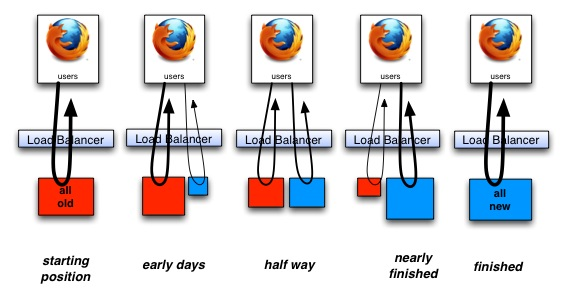
\includegraphics[width=\textwidth]{strangulation}
\end{figure}

Da der entwickelte Microservice keine Schnittstelle zum Web, sondern nur zum bereits bestehenden Monolithen hat, beschloss ich hier mit dem dem Strangler Pattern ähnlichen Prinzip der Feature Toggles\cite{fowler:featuretoggle} zu arbeiten. Statt mit einem Load Balancer, wird mit Hilfe des Ruby Flipper Gems\cite{flipper} nach und nach mehr Last auf den neu entstehenden Service zu verteilt.~\cite[vgl.][]{Hammant:Strangler}
Feature Toggles zeichnen sich dadurch aus, das über einen ``Schalter'' im Code gesteuert wird ob Requests zum neuen oder zum alten Feature geleitet werden. Beim Flipper Gem wird das Feature hier anhand einer \textit{Flag} in der Datenbank nur für bestimmte Nutzer aktiviert. So können beispielsweise für bestimmte Nutzer, zum Beispiel zunächst nur der Entwickler des neuen Features, der neue Dienst aktiviert werden, während alle anderen Nutzer noch den alten Service nutzen können. Dies dient zum Einen dem Testen des neuen Services auf Fehler, zum Anderen zur Evaluierung von dessen Performance.
Hierzu wird die zentrale Schnittstelle des QueryExecuters geschaffen. Die bestehende Schnittstelle zu MongoDB wird abstrahiert und um eine weitere, für den neuen Service, ergänzt. Diese von den beiden Klassen gebotenen Schnittstellen sind identisch. Der QueryExecuter verteilt lediglich anhand der Flipper Logik an den neuen Microservice oder den bestehenden Code.

Eine Beispielimplementierung zur Verwendung des Flipper Gems lässt sich so abbilden:
\begin{lstlisting}[language=Ruby]
def query_layer
  if api_activated?
    @query_layer = prophet
  else
    @query_layer = mongo
  end
end

def api_activated?
  flipper[:prophet_api].enabled?(querying)
end
\end{lstlisting}
Der Query Executer fragt hier lediglich ab ob für das Querying Objekt in der Datenbank der Flipper für den neuen Microservice gesetzt ist. Ist dies der Fall, wird als Query Ebene der ProphetQuerier, ansonsten der MongoQuerier zurückgegeben.

Da die Nutzerprofile noch auf Seiten der Verwaltung der Nutzer selbst in der Hauptanwendung benötigt werden, werden hier jedoch nicht alle Events abgefangen. Lediglich die, die das Querien im Bereich des Samplings betreffen. Um Datenkonsitenz zu gewährleisten, werden einmal täglich alle veränderten Daten in den Microservice geupdated. Da sich Nutzerdaten nicht häufig ändern und sich unter 100 Nutzer am Tag registrieren, reicht dies aus um ausreichend gute Query Ergebnisse zu erzielen.
  \chapter{Implementierung aufbauend auf bestehenden Technologien, REST API und Continuous Delivery}

\section{Sinatra und PostgreSQL zur Optimiertung des bestehenden Technologiestacks}
Wie bereits in vorangegangenen Kapiteln beschrieben, bieten Microservices die Möglichkeit zum optimierten Einsatz von Technologien. Für die zu entwickelnde Anwendung gab es diverse Optimierungsmöglichkeiten. Hier sollte zum Einen insbesondere auf die Wahl der Datenbanktechnologie, zum Anderen vor Allem auf die Wahl des Frameworks geachtet werden.

\subsection{Wahl des Webframeworks}
Die Hauptanwendung ist im Ruby Framework Ruby on Rails\cite{rails} entwickelt worden. Ruby on Rails ist jedoch als Framework zu \textit{heavy-weight} und mit zu viel Overhead verbunden, als das es sich für einen schnellen, minimalistischen Microservice eignen würde. Ruby on Rails ist an erster Stelle für monolithische Anwendungen entwickelt.~\cite[][]{rails:doctrine}
Hierbei ist nicht nur die Performance entscheidend, sondern auch die Struktur des Codes. Rails als traditionelles Model-View-Controller Framework\cite[][]{wiki:mvc} eignet sich somit vor Allem auch nicht aufgrund seiner Struktur. Die minimalistischere Rails API Variante\cite{rails:api} hat zwar einen geringeren Overhead als Rails, für einen geschwindigkeitsorientierten Microservice bieten sich weitere Optimierungen jedoch an.

\begin{figure}[!ht]
    \centering
    \caption{Geschwindigkeitsvergleich Rails, Rails API und Sinatra \cite{newrelic:soa}}
    \label{fig:speed}
    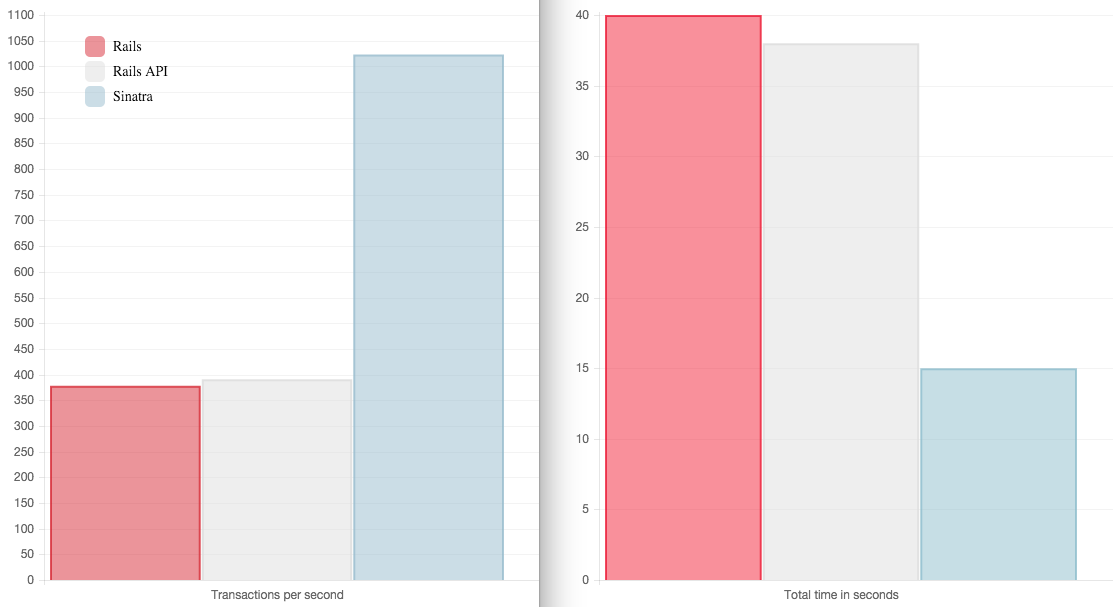
\includegraphics[width=\textwidth]{rails_sinatra}
\end{figure}

Alternativen bilden sogenannte Microframeworks\cite{wiki:micro}. Microframeworks zeichnen sich im Gegensatz zu full-stack Frameworks dadurch aus, das viele der Funktionen nicht Teil des mitgelieferten Umfangs sind. In den meisten Sprachen gibt es diverse Microframeworks, wie z.B. Flask\cite{flask} für Python, Express\cite{expressjs} für Node, Sparkjava\cite{sparkjava}, oder das Sinatra Framework\cite{sinatra} für Ruby. Die Sprache Go\cite{golang} kommt bereits mit gut ausgebauten net/http Paketen und umfasst dadurch die meisten üblichen Funktionen schon ohne Framework.

Zwar gibt es Geschwindigkeitsunterschiede in diesen Frameworks\cite[vgl.][]{frameworks}, im Vergleich zu klassischen full-stack Frameworks sind diese aber unerheblich. Da die Datenbank in der bestehenden Anwendung den größten Flaschenhals bildet (FIX STATS), muss hier nicht zwangsläufig das beste Framework gewählt werden. Stattdessen sollte auf die bestehende Firmenstruktur geachtet werden. Da fast die gesamte Backendtechnologie bisher mit der Programmiersprache Ruby entwickelt ist und es somit keine anderen im Produktionsbetrieb eingesetzt wird, wäre die Integration einer neuen Programmiersprache in das Unternehmn mit nicht unwesentlichen Kosten verbunden. Vor Allem, da der neue Microservice auch mit einem komplett eigenen Produktionssetup verbunden ist, stellt eine in der Firma bisher unbekannte Programmiersprache eine ganz eigene Herausforderung dar. Um die Wartbarkeit des Systems hoch zu halten und die Risiken für den Betrieb zu minimieren, entschied ich mich daher auch im neuen Microservice die Programmiersprache Ruby einzusetzen. Da das Framework Ruby on Rails überproportioniert ist und nicht den Anforderungen entspricht, entschied ich mich für den Einsatz des Ruby Frameworks Sinatra. 
Sinatra ist nach Ruby on Rails das mit Abstand beliebteste Ruby Framework\cite[vgl.][]{ruby2015} und wird daher von den meisten Ruby Web Tools unterstützt.

Wie bereits erwähnt, ist Sinatra ein sogenanntes Microframework. Sinatra selbst lässt also viel Raum für Konfiguration, unterstützt jedoch in den wesentlichen Zügen der Webentwicklung. Sinatra erleichtert so zum Beispiel das Routing enorm. Hier kann schnell eine Routing Struktur erschaffen werden, die Definition von Routen und deren Antworten ist sehr komfortabel und schnell einzurichten. Sinatra ist vor Allem auch nicht darauf ausgelegt in Antworten HTML zu rendern, so kann leicht eine JSON Response definiert werden.
Eine Route zum Anlegen von Resourcen kann z.B. so definiert werden:
\begin{lstlisting}[language=Ruby]
class SomeController < Sinatra::Base
  post '/resources' do
    data = JSON.load(request.body.read)
    [...] # some actions to save the resource
    # return appropriate 201 code
    [201, { data: `success' }.to_json }]
  end
end
\end{lstlisting}

Weiterhin erleichtert Sinatra das Betreiben eines Webservers und bietet eine Schnittstelle zum Ruby Standard Webserver Interface Rack\cite{rack}. Hier wird dem Entwickler viel Arbeit abgenommen. Viele Tools zum Betreiben von Webservices, z.B. im Bereich des Monitorings oder des Loggings unterstützen ebenfalls das Sinatra Framework. So bringt Sinatra also nicht viel Overhead \textit{out of the box}, bringt aber die Möglichkeit zur Nutzung vieler praktischer Erweiterungen.

Als Webserver wählte ich den Ruby Webserver Puma\cite{puma}. Puma ist ein Webserver mit verhältnismäßig geringem Speicherverbrauch, dadurch bietet er sich vor Allem für den Betrieb eines Microservices an.

\subsection{Datenbanktechnologie}
Da die Datenbank das scheinbar größte Problem der Performance in der bestehenden Anwendung bildet, ist es hier dringend notwendig die eingesetzte Technologie zu überdenken. Zwar ist MongoDB von der Idee her keine schlechte Wahl für die Userprofile, die Art wie Profildaten abgefragt werden, passt aber nicht gut zum dokumentorientierten Ansatz von MongoDB.
Die Schemalosigkeit von MongoDB in Zusammenarbeit mit den recht variablen Profilen war ursprünglich der Hauptgrund diese Technologie einzusetzen. Nutzerprofile sind stark unterschiedlich, viele mit ja beantworteten Fragen führen zu weiteren Fragen (z.B. ``Haben Sie Kinder?'', ``Wie viele Kinder haben Sie?'', ``Wie alt ist Kind x?''). Hierbei bietet es sich durchaus an MongoDB mit seiner Embedded Document Struktur zu benutzten, statt unzählige 1 zu n Beziehungen zu verwalten.
Bei der Abfrage der Daten verspricht MongoDB Geschwindigkeitsvorteile, wenn man einzelne Dokumente aus der Datenbank erhalten möchte. So kann zum Beispiel die Struktur einer Powerpoint Präsentation wie folgt abgebildet werden:
\begin{lstlisting}[language=Ruby]
{
    presentationId: 1,
    title: "A Presentation",
    author: "me",
    slides: [
        {
            slideId: 1,
            slideOrder: 1,
            elements: [
                {
                    elementId: 1,
                    elementXPos: 100,
                    ...
                },
                ...
                }
            ]
        },
        ...
    ]
}
\end{lstlisting}
Eine Präsentation kann nun mit nur einer Abfrage, ohne jegliche Joins aus der Datenbank geladen werden. Die ganze Präsentation kann vorgerendered werden und die Anwendung zur Erstellung oder Präsentation von Präsentationen ohne weiteres Nachladen genutzt werden. Hier liegt MongoDB's Stärke: Strukturen können in ihrer natürlichen Form abgebildet werden und dokumentorientiert schnell aus der Datenbank geladen werden.
So ist auch der Aufbau der Profile konzipiert worden. Für die Verwaltung der Daten und für die Pflege der Profile durch die Nutzer ist dieser Aufbau durchaus angebracht.
Beim Erstellen einer Query und dessen Ausführung über die Gesamtpopulation ist dieser Aufbau jedoch nicht optimal. Hier sind nie alle Profilfelder eines Nutzers relevant, sondern lediglich ein Querschnitt über alle Nutzer. Queries sehen in der Regel wie folgt aus:
\begin{lstlisting}[language=Ruby]
{
    "profile.participations.response_rate.value": {
        "$lt": 0.3
    },
    "profile.basic.locale.value": {
        "$in": ["de", "de-AT"]
    },
    "profile.basic.age.value": {
        "$gt": 21,
        "$lte": 100
    }
}
\end{lstlisting}

Hier wird auf eine verhältnismäßig geringe Zahl von Profilfelder, meist weniger als 10, über die gesamte Population gequeried. Weiterhin werden dann nicht gesamte Nutzerobjekte zurückgegeben, sondern lediglich die Anzahl der passenden Nutzer, deren Ids oder Antwortraten. Die MongoDB Query Struktur ist dafür schlichtweg nicht optimiert.

Hinzu kommt, dass MongoDB Datenbanken auf 64 Indizes beschränkt sind\cite{mongo:indexlimit}. Da Nutzerprofile in Nutzern eingebettet sind, gehen für die Verwaltung der Nutzer zum Login schon diverese Indizes verloren. Bei der verhältnismäßig hohen Komplexität der Profile, mit 176 Feldern, reicht dieses Limit nicht aus.
Weiterhin sind Ansätze wie ``Index Intersection'' und ``Partielle Indizes'' in MongoDB relativ neue Konzepte und noch nicht voll ausgereift\cite{mongo:indexintersection}\cite{mongo:partialindexes}.
Zwar gibt es besondere Häufungen der Queries bei bestimmten Feldern und diese sind auch durch Indexe abgedeckt, vor Allem aber die Queries auf die anderen Felder verlangsamen die Anwendung erheblich.

Hier besteht schlicht eine Diskrepanz zwischen den Queryanforderungen. Zum Einen wird hier dokumentenorientiert, zum Anderen spaltenorientiert gearbeitet.
Die Pflege der Nutzerprofile durch die Nutzer geschieht dokumentorientiert. Für die Nutzer ist immer genau ein Nutzerprofil relevant, nämlich ihr eigenes. Das Nutzerprofil wird in seiner Gesamtheit aus der Datenbank angefragt, verändert und wieder abgespeichert.
Das Nutzersampling hingegen geschieht spaltenorientiert. Über die Gesamtheit aller Nutzer wird eine bestimmte Menge von Spalten abgefragt und anschließend eine Spalte (z.B. die ids oder die Antwortraten der Nutzer) aus der Datenbank geladen.
% (FIX TOO ABSOLUTE, it's not column oriented after all)
Ein Ansatz diese Diskrepanz zwischen Nutzersampling und Profilpflege zu lösen, bietet die Command Query Responsibility Segregation (CQRS).~\cite[][]{fowler:cqrs} Gemäß der Anforderungen verschiedener Services bietet es sich hier an, die Darstellung von Daten, die theoretisch identisch sind, auf verschiedene Anwendungfälle zu optimieren. Auf Code Ebene können zum Beispiel separate Models genutzt werden um die Daten in individuelle Repräsentationsformen zu bringen. Auf Ebene der Datenbank kann ein komplett anderes Schema zur Repräsentation der Daten genutzt werden.

\begin{figure}[!ht]
    \centering
    \caption{Aufspaltung zur Lösung der Anforderungsdiskrepanz}
    \label{fig:orientationsplit}
    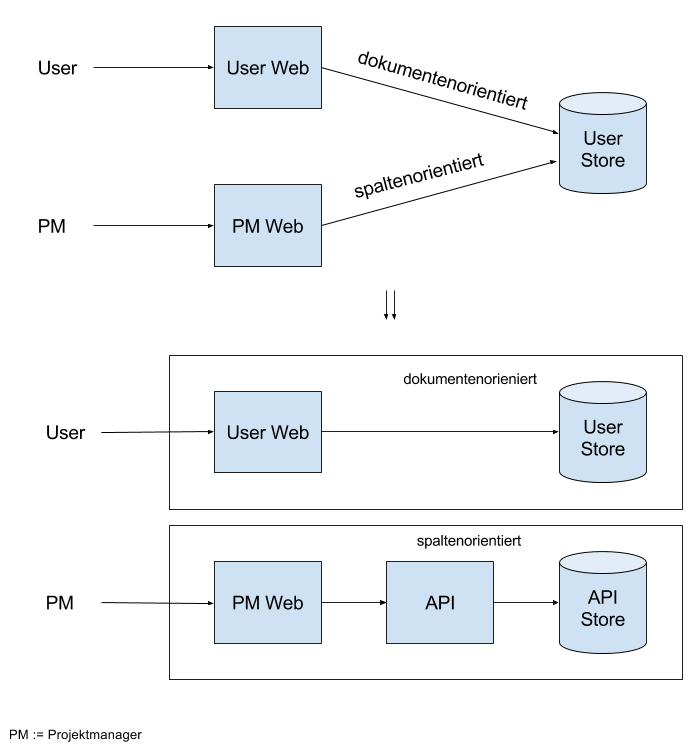
\includegraphics[width=\textwidth]{orientation_comparison}
\end{figure}

Weiterhin führen Änderungen der Nutzerprofile in MongoDB auch immer zu einem \textit{write-lock}. Auch wenn dieser noch so kurz sein mag, er behindert doch immer das gleichzeitige Auslesen der Daten. Auch das spricht für eine neue, separate Datenbank zum Lesen der Daten für Samplingzwecke.

Aufgrund der offensichtlichen Mängel im Schema im Bezug auf die Nutzerqueries bot es sich an, die Datenbanktechnologie zu wechseln und stattdessen eine SQL Datenbank zu verwenden. Im Gegensatz zum Wechsel der Programmiersprache, stellt der Einsatz einer anderen Datenbanktechnologie im konkreten Fall keine große Hürde dar. Im Betrieb besteht bereits eine MySQL\cite{mysql} Datenbank als Data Warehouse und eine PostgreSQL\cite{postgres} Datenbank für eine für einen Kunden betriebene Anwendung. Daher besteht Erfahrung sowohl in der Entwicklung mit, als auch dem Betrieb von SQL Datenbanken.
Ich entschied mich für den Einsatz einer PostgreSQL Datenbank. PostgreSQL bietet hier die Möglichkeit eine spaltenorientierte \textit{Engine} zu nutzen\cite{postgres:column}. So kann zwar im Betrieb auf bekannte SQL Technologien gesetzt werden, Optimierungsmöglichkeiten in Richtung Spaltenorientiertheit sind dennoch möglich.

Die Hauptaufgabe besteht nun darin, die bestehende, verschachtelte Struktur der MongoDB Datenbank in ein SQL Format zu übersetzen.
In \autoref{fig:fields} sind die bisher eingesetzten Ruby Klassen zur Abbildung der MongoDB Datenstruktur abgebildet. 

\begin{figure}[!ht]
    \centering
    \caption{Vereinfachtes Klassendiagramm zur Darstellung der vorhandenen Profilfelder}
    \label{fig:fields}
    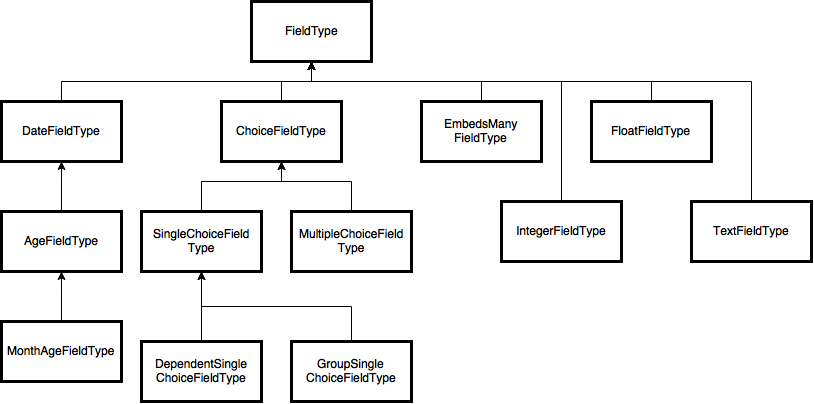
\includegraphics[width=\textwidth]{field_types}
\end{figure}

Eine Herausforderung bilden hier vor Allem die Felder der Klasse ChoiceFieldType. Die anderen Felder können problemlos in eine flache Struktur überführt werden. Für Choice Felder, sollte nun gemäß der Normalisierung von Datenbanken (FIX WELCHE NORMALFORM? QUELLE) eine eigene Tabelle mit Relation angelegt werden. Die MultipleChoice Felder müssten weiterhin mit einer `has-many' Relation abgebildet werden, was zu vielen Joins bei Queries führen würde. Da Joins im Allgemeinen verhältnismäßig langsam sind (FIX QUELLE), ist dies in Anbetracht der Aufgabenstellung ein Problem. Da die Datenbank im Microservice jedoch lediglich zu möglichst schnellen Abfrage der Daten, nicht aber zur Pflege und Organisation der Daten genutzt wird, ist es hier vertretbar eine denormalisierte Struktur zu wählen. So entschloss ich mich für den Einsatz von Bitstrings. Jede Auswahlmöglichkeit wird hier durch ein Bit repräsentiert. So kann zum Beipsiel die Mehrfachauswahl von Städten in Berlin, mit den drei Auswahlmöglichkeiten Hamburg, Berlin und München, auf einen drei Bit langen Bitstring abgebildet werden. Der Bitstring `010' in der Datebank bedeutet dann, dass nur die Option Berlin, nicht aber die Optionen Hamburg und München ausgewählt wurden. Dies spart zum Einen Platz in der Datenbank, zum Anderen reduziert es den Einsatz von Datenbankjoins. Es muss natürlich ein Overhead beim Übersetzen der alten Queries in ein Bitstring Format eingeplant werden. Weiterhin wird hier eine Kopplung zwischen Code und Datenbank eingeführt. Wenn sich die Optionen in der Datenbank ändern, muss immer zusätzlich zu allen anderen Stellen diese eine Stelle im Code aktualisiert werden.

Eine weitere Schwierigkeit stellen hier die EmbedsMany Felder dar. Auch hier ist eine `has-many` Relation notwendig, diese kann aber nicht, wie bei sich wiederholenden Auswahlfeldern, durch einen Bitstring ersetzt werden. (FIX MORE STUFF)

%(FIX NOBODY CARES? TOO MUCH GELABER??)

Zusätzlich zur relationalen Datenbank setzte ich in der Entwicklung weiterhin Redis\cite{redis} als Zwischenspeicher ein. Redis ist ein in-memory data store, der sowohl zu Datenbankzwecken, als auch zu caching Zwecken genutzt werden kann. Da die Daten ausschließlich im Arbeitsspeicher des Systems abgelegt werden, können hier sehr hohe Geschwindigkeiten erreicht werden.
Zunächst überträgt die Hauptanwendung in Form eines POST requests die Query. Diese wird dann in Redis gespeichert. Die errechneten Queryergebnisse werden dann ebenfalls in Redis gespeichert. Die Ergebnisse können dann jederzeit von der Hauptanwendung abgefragt werden. Außerdem ist es möglich und perspektivisch geplant, die Geschwindigkeit von Redis für das Caching zu nutzen. Es kann überprüft werden ob übertragene Queries bereits bekannt sind und anhand dessen Alters die Ergebnisse übernommen werden. Weiterhin kann hier Performance gewonnen werden, da keine langfristige Persistenz gefordert ist. So kann Redis einzig und allein im Arbeitsspeicher speichern und muss nicht, wie sonst üblich, jede Änderung auf der Festplatte speichern.\cite{redis:faq}

%(FIX FIRST I SAY ONLY IN-MEMORY, THEN I SAY ALSO ON DISK)

\subsection{Architektur des Microservices}
Wie bereits beschrieben, handelt es sich beim entwickelten Microservice hauptsächlich um eine Query Schnittstelle. Der Overhead soll hier möglichst gering gehalten werden um die Geschwindigkeit zu optimieren.

Da die bereits existierende Datenbank, aus den bereits beschriebenen Gründen weiter in der Betriebsawendung erhalten bleibt, bietet es sich an, zur Abfrage der neuen Datenbankfelder, die alten Feldnamen an den Microservice zu übergeben.
Die bestehende Schnittstelle zu MongoDB bietet hier eine praktische \textit{.to\_json} Methode. Mit dieser kann eine Query leicht in ein gut übertragbares Format überführt werden. Eine erstellte Abfrage auf alle Nutzer, die als Sprache deutsch angegeben haben:

\begin{lstlisting}[language=Ruby]
User.where(:'profile.basic.locale.value' => 'de')
\end{lstlisting}

\noindent kann so leicht in ein JSON-Format überführt werden:

\begin{lstlisting}[language=Ruby]
User.where(:'profile.basic.locale.value' => 'de').selector.to_json
=> { "profile.basic.locale.value": "de" }
\end{lstlisting}

\noindent So bildet das Übersetzen der übergebenen Feldnamen einen wesentlichen Teil des entwickelten Microservices.
Diese Kopplung zwischen den Services ist zwar grundsätlich nicht ideal, aber im konkreten Anwendungsfall durchaus sinnvoll. Schließlich werden beide Datenbanken weiterhin parallel verwendet und die Umstellung soll mit einem möglichst geringen Aufwand durchgeführt werden.
Es bietet sich jedoch an, in der Zukunft einen zentralen Punkt zur Pflege der Übersetzungen der Feldnamen einzurichten, um die Aktualität der Übersetzungen zu garantieren. Eine nur im Microservice verwaltete Übersetzung kann bei neu hinzugefügten Feldern in der MongoDB Datenbank leicht vergessen werden und schnell \textit{outdated} sein.

Einen weiteren wesentlichen Bestandteil bildet das Handhaben des übergebenen JSON Strings. Dieser wird im ersten Schritt anhand einer JSON Schema\cite{jsonschema} Definition validiert. So wird sichergestellt das er wohlformattiert ist und den gestellten Anforderungen entspricht. Hier kann vor dem Schritt des wirklichen Parsens ggf. noch einmal Last reduziert werden. War die Validierung erfolgreich wird der übergebene JSON String geparsed. Hierzu habe ich einen Parser entwickelt, der das übergebene MongoDB JSON Format in eine PostgreSQL kompatible Notation überführt. Schnell wird jedoch deutlich, dass es jedoch auch relati komplexe Querykonstrukte gibt. Da wäre zum Einen der Einsatz von Vergleichsoperatoren. Hier können leicht auch solche Queries entstehen:

\begin{lstlisting}[language=Ruby]
User.where(
    :'profile.basic.locale.value'.nin => ['de', 'de-AT', 'de-CH'],
    :'profile.automotive.car_amount.value'.gt => 3,
    :'profile.automotive.car_amount.value'.lte => 10
).selector.to_json
=> 
{
    "profile.basic.locale.value": {
        "$nin": ["de","de-AT","de-CH"]
    },
    "profile.automotive.car_amount.value": {
        "$gt": 3,
        "$lte": 10
    }
}
\end{lstlisting}

\noindent Dies muss der Parser also auch übersetzen können. Im gleichen Schritt werden, neben dem Parsen, auch die Datenbankfeldnamen übersetzt.

\section{Schaffung einer standardisierten REST Schnittstelle}
Einen entscheidenden Unterschied zwischen Microservice Architektur und monolithischer Entwicklung, bildet die Schnittstelle zwischen den Anwendungsteilen. Während im Monolithen simple Code Calls stattfinden, muss für die Kommunikation zwischen verschiedenen Servies zunächst ein geeignetes Protokoll zum Austausch gefunden werden.
Da hier eben kein durch die Programmiersprache vorgeschriebener Standard besteht, ist es wichtig ein geeignetes Austauschformat zu definieren.
Um Änderungen sowohl im Client, also auch im Service möglich zu machen, sollten keine sprachgebundenen Technologien eingesetzt werden. Somit kann sichergestellt werden, das möglichst geringe Änderungen anfallen, sollte ein neuer Client oder Änderungen am bestehenden System zum Einsatz einer neuen Programmiersprache führen.

Eine populäre Schnittstellentechnologie ist der Einsatz von Remote Procedure Calls (RPC)\cite{rpc}. RPC verfolgt das Hauptziel, Remote Calls wie lokale Aufrufe wirken zu lassen. Dies ermöglicht es schnell Server-Client Anwendungen zu entwickeln. Zwar sind RPC Lösungen häufig technologiegebunden\cite[vgl.][Seite 46]{newman2015building}, es gibt jedoch auch diverse Lösungen die verschiedene Technologien unterstützen. Ein großer Nachteil von RPC wird jedoch bei komplexeren Anwendungen auffällig: Remote Calls sind keine Lokalaufrufe.\cite[][Seite 47]{newman2015building} Zwar erlaubt RPC es durch ``verstecken'' der Implementierungsdetails, schnell einfache Client-Server Anwendungen zu entwickeln, mit der Zeit wird aber deutlich, dass mitunter feinere Entwicklungsmöglichkeiten notwendig sind. Hier fehlt es dann oft an besserer technologischer Kontrolle.

Eine Alternative zu RPC, die vor Allem in den letzten Jahren an Popularität gewonnen hat, ist der Representational State Transfer (REST). Im Gegensatz zu RPC, das ursprünglich für Verteilte Systeme innerhalb eines Netzwerkes oder Netzwerkverbundes entwickelt wurde\cite{rpc:history}, ist REST eng an das Internet gekoppelt\cite[vgl.][Seite 49]{newman2015building}. Nicht zuletzt deswegen wird REST, trotz relativer Protokollunabhängigkeit, meist mit dem Hypertext Transfer Protocol (HTTP) verwendet\cite[vgl.][Seite 50]{newman2015building}. Die prominenten HTTP Verben POST, GET, PUT und DELETE lassen sich direkt zu den CRUD Operationen Create, Read, Update und Delete übersetzten. Eine REST Grundlage stellt die methodische Unabhängigkeit von Ressourcen dar. Methoden sollten sich auf allen Ressourcen gleich verhalten. So kann mit Hilfe der HTTP Verben durch verschiedene Request auf eine Ressource, unterschiedliche Handlungen abgebildet werden. Statt die Methoden $createResourceX$, $readResourceX$, $updateResourceX$ und $deleteResourceX$ zu unterscheiden, kann eine einfache und abstrakte Form der Art $VERB\ RESSOURCE$ genutzt werden um alle Methoden abzubilden. So können Methoden auf Queries also durch simple HTTP Request wie $POST\ /queries$ und $GET\ /queries$ eindeutig abgebildet werden. Ein weiterer Vorteil der relativen Nähe zu HTTP, ist gute Unterstützung dieser Technolgie. Viele Technoligien die mit HTTP zum Einsatz kommen, wie z.B. Caching und Load Balancing können leicht auch mit REST eingesetzt werden\cite{rest:loadbalancing}.

Weiterhin ist REST in der Wahl des eingesetzten Austauschformats frei\cite[][Seite 53]{newman2015building}. Populäre Möglichkeiten sind hier z.B. JSON oder XML. Da die bisherige Datenbankschnittstelle einen direkten Export zu JSON bietet, bietet es sich an diese hier einzusetzen. Generell ist der Support von JSON in Ruby sehr gut. Außerdem bietet auch die eingesetzte Datenbankschnittstelle\cite{sequel} für PostgreSQL gute JSON Unterstützung.

Da das eingesetzte JSON Format frei wählbar ist und REST ebenfalls wenig Ansprüche an die Form der Daten stellt, bietet es sich hier an, unterstützend eine Technologie zur Definition des JSON Formats einzusetzen. Hier gibt es zum Beipsiel JSON Schema. JSON Schema erlaubt es die erwartete Struktur der übertragenen Daten, z.B. bei POST Requests, abstrakt festzulegen. Dies erlaubt zum Einen leichte Nachvollziehbarkeit der Schnittstelle, zum Anderen eine automatische Validierung der übergebenen Daten. So muss nicht mit dem Parsen der Daten begonnen werden, ohne das vorher sichergestellt ist, das diese semantisch korrekt sind.

Weiterhin ist es wichtig, die erstellte API gut zu dokumentieren. Hier gibt es ebenfalls gute Tools die eingesetzt werden können. Ich nutze hierzu die RESTful API Modelling Language (RAML)\cite{raml}. RAML erlaubt es eine Schnittstelle in einem Maschinen-lesbaren Format zu dokumentieren. Dies erlaubt es automatisiert API Tests generieren zu lassen. So kann sichergestellt werden, dass die API Dokumentation immer auf dem aktuellsten Stand ist. Denn wenn die API, nicht aber die Dokumentation aktualisiert wird, würden hier die generierten Tests fehlschlagen. Dies ist für verteilte Systeme besonders wichtig. RAML arbeitet hierzu mit JSON Schema um Beispielrequests zu definieren. Weiterhin lässt sich mit Tools wie RAML to HTML\cite{raml2html} leicht eine interaktive, menschenlesbare Dokumentation der API erstellen. Hier finden sich dann automatisch auch die Beispielrequests und -responses der API in JSON Format. Die Dokumentation der entwickelten API ist so für Entwickler in Form einer Webseite\cite{prophetdoku} nachvollziehbar. 
Weiterhin kann über Tools\cite{ramlconsoletool} auch eine interaktive Testkonsole generiert werden, die es erlaubt die API anhand der bereitgestellten Beispiele zu Testen.

REST, vor Allem im gemeinsamen Einsatz mit JSON-Schema und RAML, bildet eine reife Technologie, die sich für den Einsatz in der API Programmierung hervorragend eignet.

%(FIX RAM console)

\section{Integration des Microservices in den Monolithen}
Wie bereits im vorangegangenen Kapitel beschrieben, beschloss ich den neuen Microservice mit Hilfe eines dem Strangler Pattern ähnlichen Prinzips in die bestehende Anwendung einzubinden.
Der Einsatz des Flipper Gems erlaubt es hierbei den bestehenden Code mit alter Datenbank, sowie den neuen Microservice mit neuer Datenbank parallel zu betreiben. Anhand der abstrahierten Schnittstelle des QueryExecuters, wird entschieden, ob ein Query auf der alten Datenbank oder dem neuen Service stattfindet. Das entsprechende Klassendiagramm ist in \autoref{fig:class} dargestellt.
\begin{figure}[!ht]
    \centering
    \caption{Klassendiagramm zur Verteilung zwischen bestehendem und neu geschaffenem Code}
    \label{fig:class}
    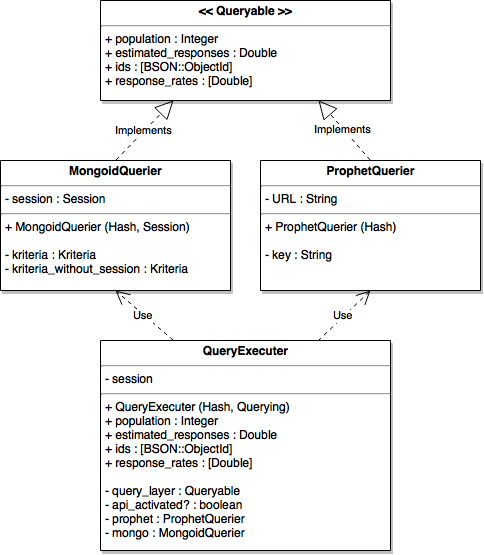
\includegraphics[scale=0.6]{klassendiagramm}
\end{figure}

Ist der Toggle aktiviert, wird zunächst per POST ein Query an den Service übertragen. Im Hintergrund initiiert der Service dann das Parsen, Übersetzen und Abarbeiten der Query. Dies geschieht asynchron. Zunächst wird die Query in Redis gespeichert und der generierte Zugriffsschlüssel zurückgegeben.
Anhand dieses Schlüssels kann die Hauptanwendung dann die freigegebenen Ergebnisse des Querys, wie die ids der zutreffenden Nutzer, abfragen. Der Ablauf kann wie in \autoref{fig:sequenz} visualisiert werden.

\begin{figure}[!ht]
    \centering
    \caption{Sequenzdiagramm zum Profilqueryen bei aktiviertem Flipper}
    \label{fig:sequenz}
    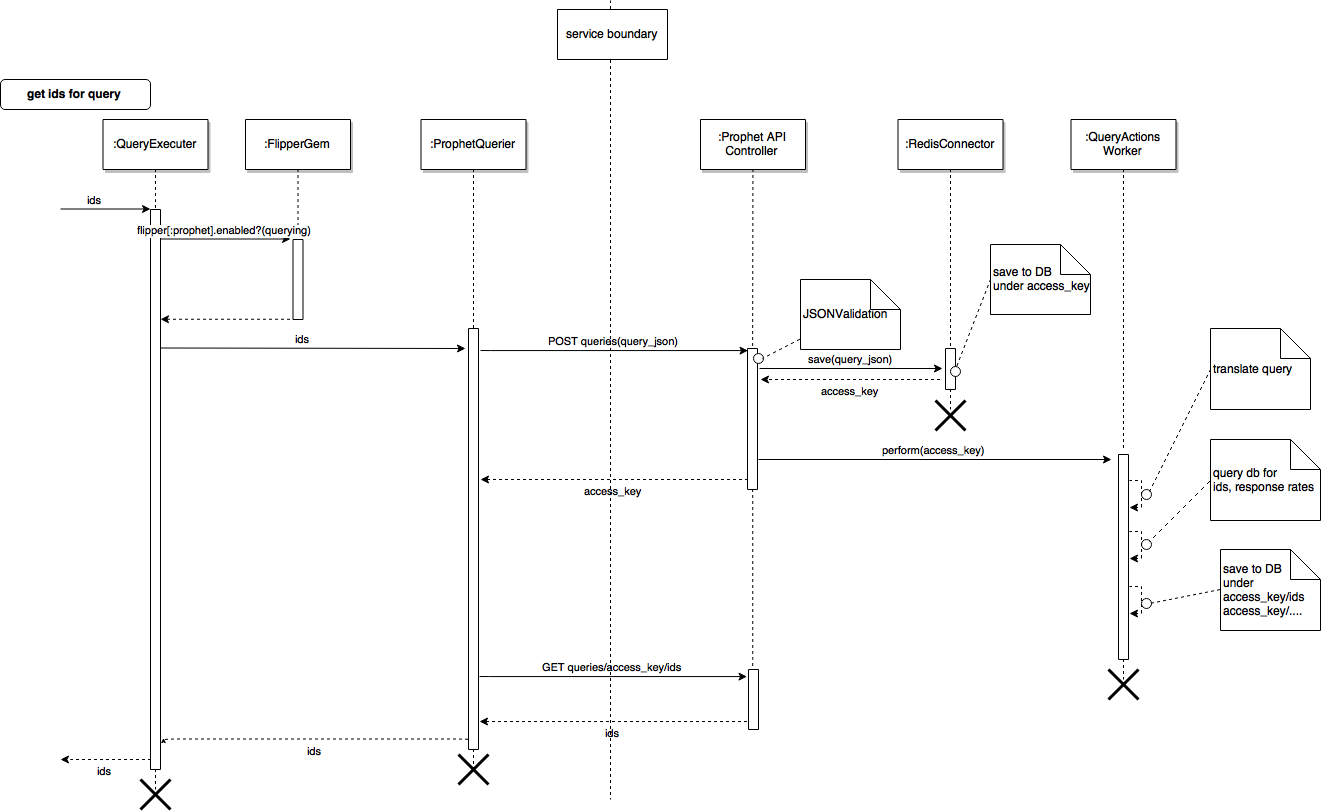
\includegraphics[width=\textwidth]{prophet_sequenz}
\end{figure}

Hier ist insbesondere das Fehlerhandling zu beachten. Es gibt hier diverse Fehlerquellen die den Ablauf beeinträchtigen können. Zum Einen kann die Query fehlerhaft sein. 
Tritt bei der JSON-Schema Validierung ein Fehler auf, wird hier ein HTTP 422 Statuscode zurückgegeben. Per Definition der Internet Engineering Task Force (IETF)\cite{ietf:424} handelt es sich hierbei um eine ``Unprocessable Entity''. Die übertragenen Daten können also nicht verarbeitet werden.
Da das Parsen der Query asynchron geschieht und die Query vorher nur Anhand von JSON-Schema validiert wird, kann eine fehlerhafte Query, beispielsweise durch illegale Datenbankfeldnamen, erst nach Antwort mit Zugriffsschlüssel erkannt werden. Geschieht dies, muss beim Abfragen der Daten von der API ein eindeutiger Fehlercode zurückgegeben werden. Es muss unterschieden werden können zwischen invaliden Schlüsseln, Timeouts und illegalen Queries. Für Abfragen nach Übermittlung illegaler Queries habe ich den Fehlercode 424 gewählt. Per Definition der IETF\cite{ietf:424}, handelt es sich hierbei um eine `failed dependency'. Der Request ist also fehlgeschlagen, da ein vorheriger Request fehlgeschlagen ist. Dies ist meiner Meinung nach der am besten passende Fehlercode.
Weiterhin kann es natürlich vorkommen, dass die Daten abgefragt werden, obwohl die Query noch nicht abgeschlossen ist. Die Daten liegen schlichtweg nicht vor. Hier wird ein HTTP 428 Statuscode genutzt. Per IETF\cite{ietf:428} steht dieser Statuscode für ``Precondition Required''. Eine benötigte Kondition wurde demnach nicht erfüllt. Dieser Statuscode passt zwar nicht so eindeutig wie der 424 Statuscode, ist aber dennoch eine angemessene Antwort.
Für den Fall, dass der Zugriffsschlüssel selbst nicht valide ist, wird ein simpler 404 Fehlercode zurück gegeben.

Für den den Fehlercode 428 (Query noch nicht abgeschlossen) und sämtliche Netzwerkfehler aus dem Fehlerbereich 500 bis 511, muss sichergestellt werden, dass erneute Abfrageversuche stattfinden.
Ein populärer Ansatz für solche Situationen, ist der des ``Exponential Backoff''\cite{expbackoff}. Bereits im Ethernet Protokoll wird Exponential Backoff eingesetzt\cite{etherbackoff}. Beim Prinzip des Exponential Backoff wird die Zeit zwischen erneuten Versuchen multiplikativ immer weiter erhöht. Die Basisgröße der zeitlichen Abstände kann hier frei gewählt werden. Der zweite Versuch findet hier in der Regel fast direkt nach Fehlschlagen des ersten statt, anschließend werden die Abstände immer größer. Hier wird die Last auf den beteiligten Systemen relativ gering gehalten, eine Operation aber nicht abschließend fehlschlagen gelassen. Grundsätzlich bietet es sich jedoch an, eine Grenze für die Zahl der Fehlerversuche festzulegen (Truncated Exponential Backoff). Wenn der Abstand z.B. auf einen Tag steigt, ist ein erneuter Versuch sicherlich nur noch bedingt sinnvoll.
Alle Queries in der Hauptanwendung werden asynchron mit Hilfe von Sidekiq\cite{sidekiq} ausgeführt. Sidekiq selbst implementiert für die ausgeführten Jobs bereits das Exponential Backoff Prinzip. Sidekiq's Retries sind jedoch auf 25 Versuche limitiert, dies bildet einen Zeitraum von 21 Tagen\cite{sidekiq:errors}, was für den Anwendungfall eindeutig zu lang ist. Hier muss für die Query Aufträge ein eigenes Limit festgesetzt werden. Ansonsten eignet sich der Einsatz von Sidekiq's Exponential Backoff Prinzip jedoch sehr gut zur Behandlung von Netzwerkfehlern. 
Weitere Technologien zur Absicherung und Optimierung der Performance wurden bisher nicht praktisch umgesetzt, sollten aber für die Zukunft in Betracht gezogen werden. Hier sind insbesondere Circuit Breaker\cite{MSDN:Circuit}\cite{Fowler:Circuit} und Throttling\cite{MSDN:Throttling} zu nennen.

Ein weiteres Thema, das bisher im Rahmen der Anwendungsentwicklung nicht beachtet wurde, ist das der Authentifizierung am Microservice. Offensichtlich ist es absolut sicherheitskritisch, dass nicht ohne jegliche Authentifizierung Daten vom Service abgefragt werden können. Hierzu bieten sich diverse Vorgehensweisen an. Zum einen sollte das Zugriffsrecht auf das IP Netz der konsumierenden monolithischen Anwendung beschränkt werden. Dies ist eine einfache Möglichkeit, ein relativ hohes Maß an Sicherheit zu generieren. Weiterhin sollte... (FIX MICROSERVICE SECURITY AND AUTHENTICATION)

\section{Betrieb der Anwendung auf AWS - Betreuung, Monitoring und Scaling}
Wie bereits beschrieben, bilden die Skalierungsmöglichkeiten von Microservices einen großen Vorteil des Architekturstils. Um diesen optimal ausnutzen zu können, bietet es sich an, eine dynamische Hostinglösung zu verwenden. Hier gibt diverse Lösungen, die alle einen ähnlichen Funktionsumfang bieten. Es muss jedoch grundlegend zwischen Platform as a Service (PaaS) und Infrastructure as a Service (IaaS) unterschieden werden. 
Bei PaaS wird BLA bei IaaS wird hier BLA. FIX AUSBAU Unterschied
Zu nennen sind hier z.B. die IaaS Lösungen Amazon Web Services (AWS) und Google Compute Engine\cite{googlecompute} und die PaaS Lösungen Google App Engine\cite{googleapp} und Heroku\cite{heroku}.
Für den konkreten Anwendungsfall entschied ich mich AWS zu nutzen. AWS bietet hier vereinfachte IaaS Lösungen die PaaS ähneln, ermöglichen jedoch immer den Ausbau zu vollwertigeren Infrastrukturen.
Auf AWS nutze ich Amazon Elastic Beanstalk\cite{aws:beanstalk} zum Betreiben der Anwendung. Elastic Beanstalk (EB) nutzt intern EC2 Instanzen, baut aber eine eigene Konfigurationsschicht darauf auf. Daher muss keine gesamte virtuelle Maschine verwaltet werden, stattdessen kann die Anwendung leicht über ein Konfigurationsinterface, wie in \autoref{fig:awsui} dargestellt, gesteuert werden.

\begin{figure}[!ht]
    \centering
    \caption{AWS Beanstalk Konfigurationsinterface}
    \label{fig:awsui}
    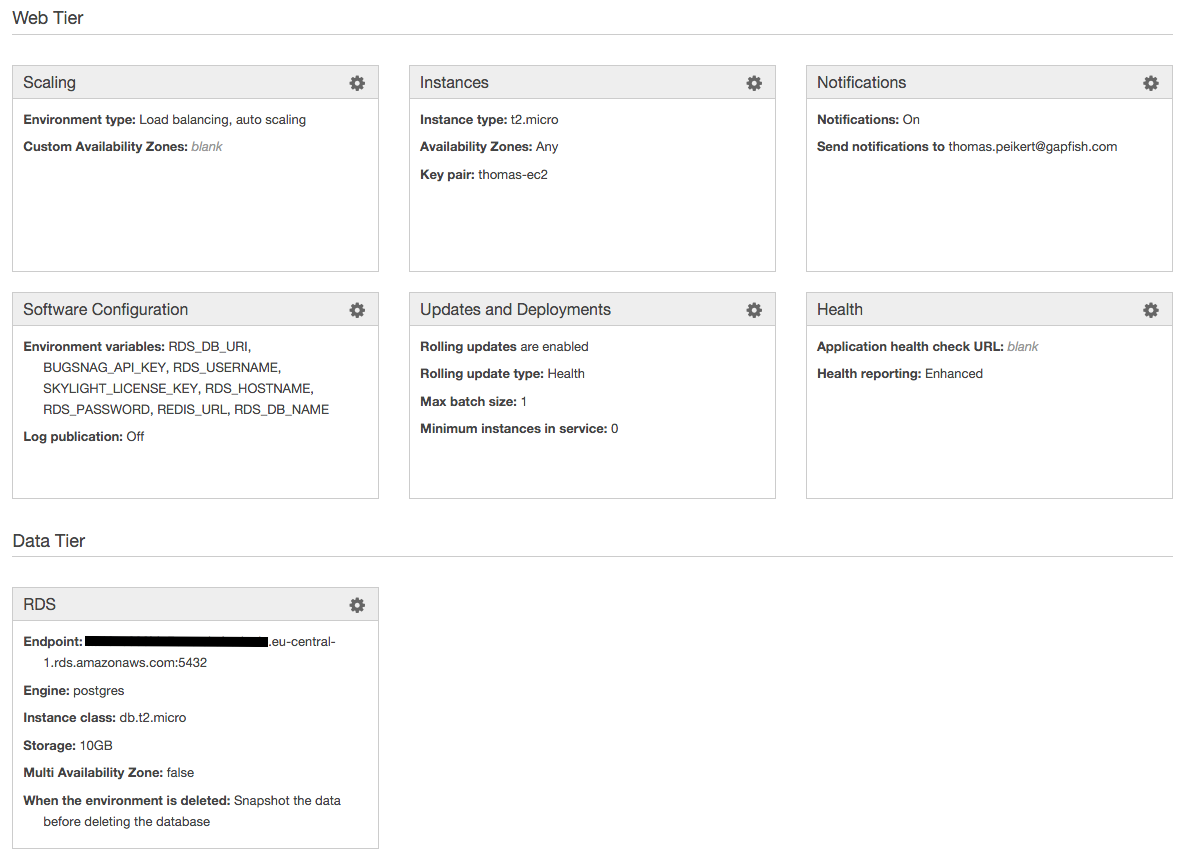
\includegraphics[width=\textwidth]{aws_config_ui}
\end{figure}
AWS EB ist selbst mit keinen Kosten verbunden, die Kosten ergeben sich ausschließlich aus den von EB genutzten Ressourcen, also die genutzten EC2 Instanzen und der reine Speicherverbrauch der Anwendung auf AWS S3. 

Elastic Beanstalk bildet hier einen Hybridansatz zwischen Iaas und Paas. Es wird lediglich eine komplette Anwendung mit Dependency Management hochgeladen und automatisiert deployt, nicht aber eine gesamte Maschine eingerichtet.
Die weiteren, von der Anwendung benötigten Ressourcen, werden jedoch, wie bei IaaS üblich, separat eingerichtet und verwaltet. Zum Einen ist dies eine PostgreSQL Datenbank und der Key-Value Store Redis. Hierfür bietet Amazon jeweils gesonderte Services zum Betrieb. Relationale Datenbanken können über den Amazon Relational Database Service (RDS)\cite{aws:rds} genutzt werden, Redis wird über Amazon ElastiCache\cite{aws:elasticache} angeboten. Beide Services bieten ebenso wie Elastic Beanstalk gute Skalierungsmöglichkeiten.

Bisher wurden die gesamte Firmenanwendung auf einem System, bei einem Hoster betrieben. Zwar gibt es durchaus separate Repositories, z.B. um eine API für die mobilen Anwendungen zu bieten, diese werden jedoch immer über das Ruby Webserver Interface Rack in die bestehende Anwendung eingebunden. So werden sie bei jedem Deploy der Hauptanwendung ebenfalls deployt. Weiterhin laufen sie im selben Prozess auf dem gleichen Server wie die Hauptanwendung. Hier ist also keinerlei separates Handling zum Monitoring notwendig. Es kann auch keinen Ausfall eines Teilsystems geben, da alle Teile zusammenhängen. Lediglich die Datenbanken und Redis laufen auf dedizierten Servern, diese werden aber im gleichen Netzwerk betrieben, somit sind zwar Teilausfälle möglich, diese werden durch ein Primary-Secondary System abgesichert, Netzwerkprobleme sind aber in der Regel ausgeschlossen. Das gesamte System kann wie in \autoref{fig:deployd} dargestellt werden.

\begin{figure}[!ht]
    \centering
    \caption{Deploymentdiagramm: Zusammenspiel aller Komponenten}
    \label{fig:deployd}
    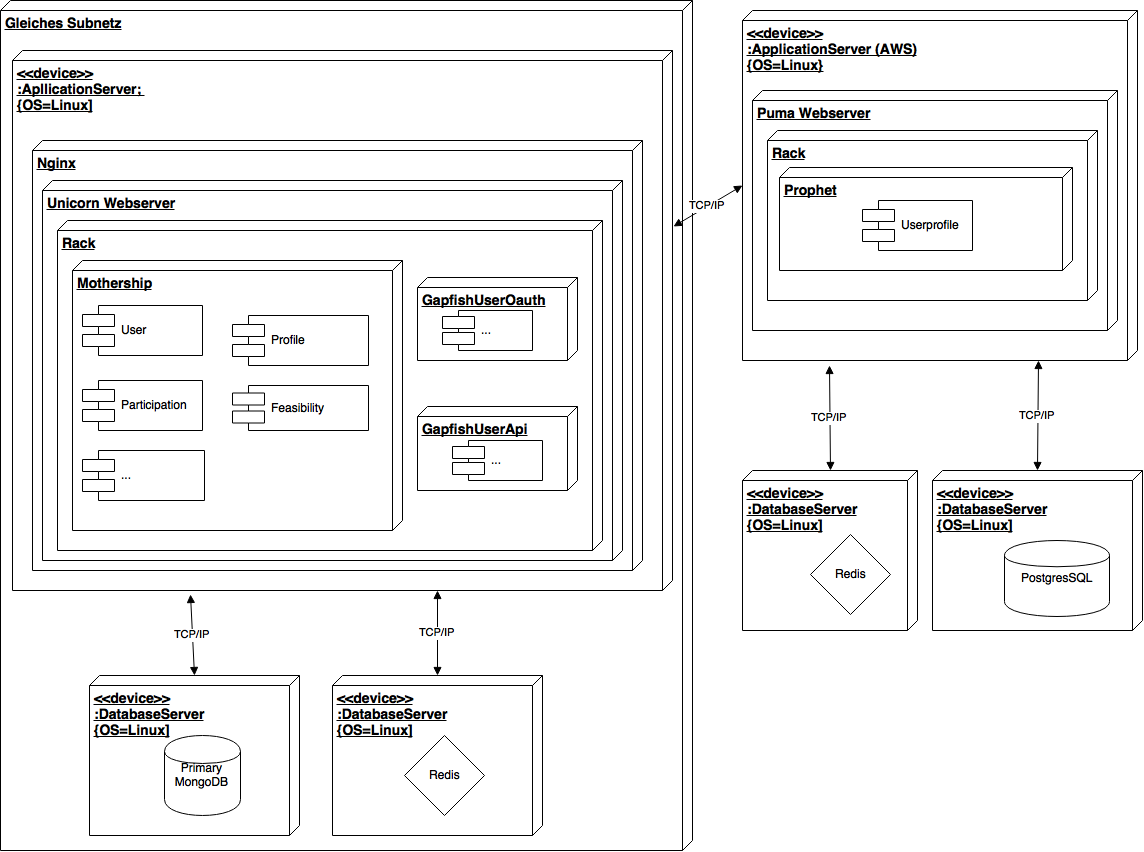
\includegraphics[width=\textwidth]{deploymentdiagram}
\end{figure}

Besonders wichtig für den Microservice ist daher das Monitoring der Anwendung und des Servers. Da hier ein von der Hauptanwendung komplett separates System betrieben wird, muss sichergestellt werden, dass zum Einen Fehler schnell erkannt und zum Anderen schnell behoben werden. 

Zum Monitoring nutze ich zum Einen Amazons eigene Monitoring Lösung, die über den Gesundheitsstatus der Anwendung informiert. Wechselt die Anwendung vom Gesundheitsstatus ``OK'' in einen anderen, werden die Entwickler direkt über eine Email informiert.

Zusätzlich zum allgemeinen Ausfallmonitoring durch Amazon, integrierte ich das Monitoring Tool Skylight\cite{skylight} in die Anwendung. Im bisherigen Betriebssetup wird aktuell NewRelic\cite{newrelic} zum Monitoring eingesetzt. Skylight zeichnet sich jedoch durch einen besonders geringen Overhead aus, was sich beim Microservice durchaus anbietet. Skylight informiert ebenfalls per Email über Ausfälle und zeichnet im Allgemeinen die Performance des Systems auf. So kann zu jedem Zeitpunkt der Vergangenheit, über Wochen hinweg, detailliert die Performance des Sytsems nachvollzogen werden. Zusätzlich zu allgemeinen Aufzeichnungen der Response Time, kann hier nach Datenbankabfragen unterschieden werden. So wird schnell deutlich, welche Anfragen besonders zeitintensiv sind und wo Handlungsbedarf oder Verbesserungsmöglichkeiten bestehen. 

Als Fehlerreporting Tool kommt im Microservice Bugsnag\cite{bugsnag} zum Einsatz. Bugsnag wird bereits als primäres Firmentool verwendet und eignet sich ebenfalls gut für kleine Anwendungen. Bugsnag zeichnet Fehler im System mit Stacktrace auf und informiert die Entwickler ebenfalls per Email.

Das Informieren über Fehler per Email ist im Unternehmen ein durchaus üblicher Weg, daher eignet sich diese Integration auch für den neuen Service. Weiterhin besteht in der Firma ein Dashboard, was zwar nicht die Performance des neuen Microservices an sich, aber die Gesamtperformance des Sampling Prozesses darstellt. Dieser umschließt alles vom Erstellen der Query, der Abfrage des neuen Services, bis hin zum Verarbeiten und Anzeigen der Queryergebnisse. So können Probleme auf dem Dashboard leicht von den Entwicklern bemerkt werden. All dies sind im Live Betrieb erprobte Techniken und eignen sich dadurch sehr gut für die Ausweitung auf neue Services.

\section{Analyse der Performance des Microservices}
Da der neue Microservice zum Zweck der Beschleunigung von Nutzerprofilqueries entwickelt wurde, ist hier insbesondere eine Auswertung der Geschwindigkeit des neuen Services angebracht. 
Zur Bewertung der Performance des neu entwickelten Microservies wurde die neue Datenbank mit Dummydaten gefüllt. Da im Rahmen der Bachelorarbeit aus Zeigründen kein vollständiges Ausformulieren des Schemas möglich war, wurden hier zusätzlich zu einigen wenigen echten Feldern, 165 Dummyspalten des Typs String angelegt. Anschließend wurden die Spalten mit 200.000 Nutzerdaten gefüllt. Dieser Datenbestand diente als Grundlage aller folgenden Performanceanalysen. Zum Vergleich dazu wurde in der Primärdatenbank Anfragen auf ein Panel beschränkt. Nutzer sind hier je nach Umfrageplatform, auf der sie sich registriert haben, in verschiedene Panels unterteilt. Das ``EC'' Panel umfasst hier ebenfalls rund 200.000 registrierte Nutzer und diente als Grundlage der Vergleiche.
Beim Vergleich der Performance muss hier grundlegend in zwei Arten der Queries unterschieden werden. Zum Einen sind dies Queries auf solche Spalten, die durch Indizes abgedeckt sind, zum Anderen auf solche Spalten, die nicht durch Indizes abgedeckt sind.

Hier muss explizit darauf hingewiesen werden das es sich bei den durchgeführten Tests um reine Performance Tests, nicht aber Load oder Stress Tests handelt.
Um die Testergebnisse möglichst repräsentativ zu halten, wurde hier im Live System getestet.\cite{msdn:perftesting} 
Da eine vollkommene Lastfreiheit des bestehenden Live Systems schlicht unmöglich ist, wurden hier Testzeitpunkte mit möglichst geringer Last gewählt. Vor Tests wurde immer explizit sichergestellt, dass aktuell keine Berechnungen o.Ä. laufen. Dies war in der Regel in den frühen Morgenstunden (vor 7 Uhr) am besten möglich.
Für den entwickelten Microservice war Lastfreiheit leicht zu garantieren, da der Zugriff, wie bereits beschrieben, über Feature Toggling kontrolliert wurde. 

Die Performance Tests wurden immer vom bestehenden Live System aus gestartet. Hierzu wurde eine SSH Verbindung aufgebaut und anschließend eine Ruby Konsole gestartet. Hier wurden direkt die QueryExecuter Subklassen des MongoidQueriers und des ProphetQueriers genutzt. Dies ist eine angebrachte Stelle zum Testen, da genau an dieser Stelle zwischen den beiden Features getoggled wird. Der restliche Ablauf ist im System identisch.

Um die Performance des Microservices messen zu können, wurde dieser leicht angepasst. Da das Fehlerhandling noch nicht ausreichend integriert ist, wurde der Microservice hier auf eine synchrone Berechnung umgestellt. Die Hauptanwendung erhält den Zugriffsschlüssel also erst, wenn die Abfrage auf die Datenbank abgeschlossen ist. Dadurch wird zwar ggf. etwas Zeit für über die synchronen Netzwerkaufrufe verloren, die Messung der echten Queryzeit ist dadurch aber erst verlässlich möglich.

Der Microservice nutzt auf AWS bisher die kleinsten Instanzgrößen, keinerlei Replikation oder Skalierung und keinerlei Indizes außer, die zum Testen angelegten. 
Hier ist davon auszugehen, dass Optimierungen, wie sie auch in der Hauptanwendung genutzt werden, also Replikationen und größere Instanzen, noch Verbesserungen erzielen können. Gerade über Indizes, die in MongoDB bereits alle in Benutzung sind, ist hier von einer Verbesserung der Performance gegenüber der Hauptanwendung auszugehen.

Zum Messen der Performance wird hier die Ruby eigene Klasse ``Benchmark'' genutzt. Sie bietet sich für einfache Zeitmessungen an. 
Es wurden diverse, für die Anwendung typische, Queries gebildet und als Selector formuliert. Jede Query wurde anschließend an die jeweiligen Klassen des MongoidQueriers und des ProphetQueriers übergeben. Abschließend wurde die Population (COUNT) und die \textit{response rates} (SELECT) abgefragt. Queries wurden jeweils 100 mal ausgeführt. Die in \autoref{fig:perftesttable} aufgelisteten Zahlen beziehen sich auf den daraus errechneten Durchschnitt einer einzelnen Query.

\begin{figure}[!ht]
    \centering
    \caption{Performance Tests diverser Queries: MongoDB vs. SQL API}
    \label{fig:perftesttable}
    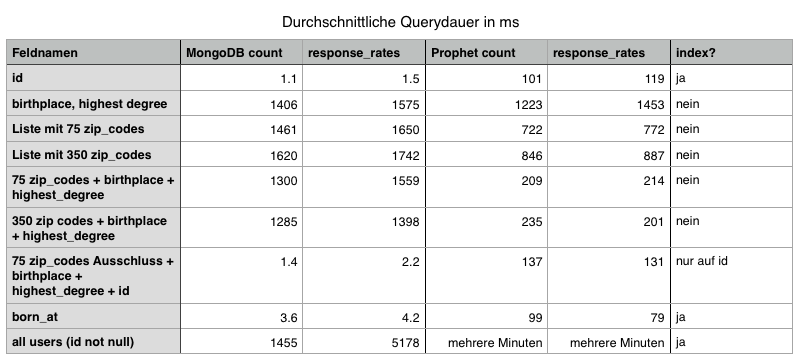
\includegraphics[width=\textwidth]{performance_table}
\end{figure}

Besonders auffällig sind die Zeitunterschiede zwischen den Abfragen der simplen Zahlen (COUNT) und dem Abfragen konkreter Daten (SELECT), wie \textit{ids} oder \textit{response rates}. Hier zeigen sich im Gegensatz zu MongoDB im Microservice keine signifikanten Zeitunterschiede. Dies ist auf die Abarbeitung der Query im Microservice zurückzuführen. Damit nur eine Query ausgeführt wird, werden hier alle erforderlichen Daten (\textit{ids}, \textit{response rates}, \textit{response rate sum} und \textit{count}) in einem Schritt aufbereitet. Es werden hierfür immer \textit{ids} und \textit{response rates} aus der Datenbank abgerufen. Anschließend werden diese gezählt und die die \textit{response rate sum} gebildet. Dadurch kommen Unterschiede lediglich durch Latenzvariation und ggf. Bilden der JSON Antwort zustande.
In jedem Fall sollte darüber nachgedacht werden, inwiefern hier Optimierungen möglich sind. Eventuell bietet es sich an, die einzelnen Schritte wie in MongoDB aufzusplitten. Hierdurch würden sich aber vier Queries ergeben. Mitunter wären hier die COUNTs dann früher bereit, im Lebenszyklus eines Projektes werden jedoch immer alle Daten benötigt, demnach macht dies nur bedingt Sinn. 

Auffällig ist hier auch das SELECT aller ids (\textit{id not null}). Hier kommt es zu extremen Laufzeiten beim Microservice. Dies ist vermutlich eher ein Problem im Code, als bei der Datenbankabfrage an sich und daher behebbar. Es scheint auf die Hohe Zahl der Daten zurückzuführen zu sein (200.000). Bei den anderen Queries wurden in der Regel bis 20.000 Ergebnisse zurückgegeben. Dies geht über die üblichen Problemgrößen in der Anwendung bereits hinaus und ist daher für den Vergleich ausschlaggebend.

Nichtsdestotrotz hat man im Microservice auch relativ hohe Queryzeiten. Bei einer Requestlaufzeit von 50ms wird hier im ersten Schritt beim asynchronen Queryen der API immer ein Fehler auftreten. Demnach wären hier immer mehrere Requests notwendig. Ggf. bietet es sich an, hier einen initialen Timeout auf Basis der durchschnittlichen Berechnungslaufzeit einzurichten, um unnötige Requests zu sparen. Ein beibehalten des synchronen Abarbeitens und direktes zurückgeben der errechneten Daten würde gegen die REST Spezifikation verstoßen und wurde daher zunächst ausgeschlossen, wäre aber für die Zukunft durchaus denkbar.

\begin{figure}[!ht]
    \centering
    \caption{Durchschnittliche Query Laufzeiten in ms: index vs no index, count vs. select}
    \label{fig:perftestgraph}
    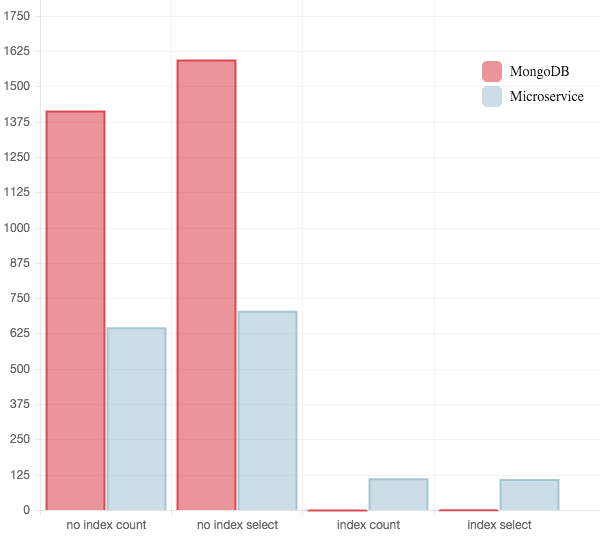
\includegraphics[width=\textwidth]{performance_graphs}
\end{figure}

Im Allgemeinen wird aber ein Trend sichtbar. Bei üblichen Queries mit normalen Resultatgrößen auf Felder ohne Indizes kann schon jetzt Zeit gewonnen werden. Dies wird nur besser, wenn hier in PostgreSQL Indizes angelegt werden. 
Auf Felder die in MongoDB bereits durch Indizes abgedeckt sind, kann hier keine Zeit gewonnen werden. Zwar sind diese Requests im neuen Service auch sehr schnell, aber der einfache Overhead durch die Netzwerkkommunikation lässt hier eine höhere Zeit zustande kommen.
Dies ist zwar nicht optimal, aber ein durchaus akzeptabler Tradeoff im Unternehmen. Wichtig ist hier eine konstant gute Performance. Die bereits erreichten Verbesserungen sind hier ein guter Anfang.
Weiterhin ist darauf hinzuweisen, dass es sich hier im bestehenden um einen fast lastfreien Zustand handelte. Unter Last im Betrieb, mit Locking der Datenbanken bei Änderungen an Userprofilen, Replication Lag und weitere Last auf der Datenbank durch andere Operationen kommen hier mitunter teilweise sehr lange Query Laufzeiten zustande. 
All dies, ebenso wie Varianzen in den Querylaufzeiten, Analyse des 95. Percentils, hinzfügen von Indizes auf PostgreSQL etc., wurden in dieser kurzen Performance Analyse nicht berücksichtigt. Sie soll nur ein generelles Gefühl für die gewonnene Performance des bei Weitem noch nicht fertigen Prototyps vermitteln.
  \chapter{Microservice Architektur als Pattern der Zukunft?}

Die Frage, ob Microservice Architektur im Betrieb eingesetzt werden sollte, lässt sich pauschal nicht beantworten. Die Voraussetzungen, um erfolgreich zu einer Microservice Architektur zu wechseln, sind individuell und vor allem von der bestehenden Anwendung und den Teamgegebenheiten abhängig. Microservices können dabei helfen viele Probleme des klassischen monolithischen Anwendungsentwicklung, insbesondere eine große, unübersichtliche Codebase, Performance-Probleme, hohe Kosten und unklare Strukturen, zu lösen. Jedoch setzt der Einsatz vieles voraus, dessen Aufbau ein langwieriger Prozess sein kann. Eine Teamstruktur, in denen sich Entwickler selbst für den Betrieb der von ihnen entwickelten Anwendung verantwortlich sehen, dynamische Serverstrukturen  zum Skalieren der Services wie sie z.B. AWS, Google Compute Engine und Heroku bieten, automatisierte Deploys und ausgereifte Monitoring-Lösungen sind für den erfolgreichen und sinnvollen Einsatz von Microservices unabdingbar.

Sollten Microservices nicht direkt zu Beginn des Softwarelebenszyklus entstehen, ist es wichtig den Übergang so kontrolliert wie möglich zu schaffen. Die Microservice Architektur stellt sicherlich keine schnelle Lösung für Probleme im Betrieb dar. Stattdessen ist sie eine längerfristige Strategie um die Organisation und Arbeit in der Firma zu verbessern \cite{newman2015building}. Wird eine bestehende Anwendung zu einer Microservice Architektur umgewandelt, bietet es sich zum Beispiel an, neu entstehende Software-Teile als Microservices zu entwickeln, um so die Codebase nicht noch weiter wachsen zu lassen. Auch besteht die Möglichkeit einen neuen Service zunächst an den bestehenden Hauptservice zu koppeln. Das \enquote{große} Framework Ruby on Rails bietet so z.B. die Möglichkeit, mit dem Microframework Sinatra entwickelte Apps in der Hauptanwendung zu \textit{mounten}. Hierdurch erhält die Subanwendung einen relativen Pfad in der Hauptanwendung und kann so wie über interne Routen angesprochen werden. Die Subanwendung kann dann mit der Hauptanwendung deployt und betrieben werden. Hierdurch können viele der initialen Herausforderungen von Microservices, wie das Monitoring, der separate Betrieb und die dynamische Skalierung der Anwendung, umgangen werden, jedoch einige der Vorzüge, wie separate Codebases und klare Strukturen bereits genutzt werden. Ebenso können hier dann z.B. auch queueing-Dienste wie Sidekiq als Kommunikationsschnittstelle dienen \cite[vgl.][]{sidekiqmessaging}. Dies erspart zunächst die Entwicklung einer vollwertigen API. Nach Aufbau geeigneter Firmenstrukturen kann die Anwendung dann mit verhältnismäßig geringem Aufwand zu einem vollwertigen Microservice ausgebaut werden. So ist man zeitlich bei der Programmierung eines Microservices nicht an dessen unmittelbaren Betrieb als solcher gebunden.

In der hier entwickelten Anwendung wurde vor allem beim Ersetzen der bestehenden Anwendungsteile durch den Microservice auf eine kontrollierte Integration geachtet. Durch Feature Toggles wurden zunächst im Betrieb nur bestimmte, explizit gewählte Queries an den Microservice gesendet. Später können dann schrittweise einzelne User freigeschaltet und prozentual, langsam eine immer höhere Zahl an Queries an den Microservice umgelagert werden. So kann nach Testen und Sicherstellen der Funktion langsam immer mehr Last auf den Microservice verschoben und so die Chance einer Überlastung und anderer unerwarteter Fehler minimiert werden.

In der hier umgesetzten praktischen Arbeit kann man den entwickelten Microservice als Erfolg betrachten. Der entwickelte Microservice ist weit mehr als nur ein Prototyp und wird nun aktiv in den Betrieb integriert. Zwar ist die Entwicklung noch nicht abgeschlossen und die parallele Anwendung mit der alten Struktur ist durchaus ratsam, die erhofften Performance Verbesserungen durch die Entwicklung der neuen Teilanwendung konnten jedoch erreicht werden. Die Transition, wenn auch noch nicht komplett abgeschlossen, läuft erfolgreich und die Struktur der Anwendung konnte, vor allem in den Augen der betroffenen Entwickler, verbessert werden. Lediglich auf der Seite der Kosten konnte keine Verbesserung erzielt werden. Dies liegt vor allem daran, dass der bisherige Hosting Plan keinerlei Dynamik vorsieht und so, trotz sinkender Last, zu keiner Kostenreduzierung führt. Die durch den neuen Service entstehenden Mehrkosten sind aber nicht höher als erwartet und somit stellt auch dies kein Problem dar.

Die Ausarbeitung von neuen Monitoring, Logging und Deploy Lösungen wurde im Rahmen der Arbeit erfolgreich umgesetzt und bereits im Unternehmen erprobt.

Aus Entwicklersicht kann man ebenfalls von einem Erfolg sprechen. Die Entwicklung eines komplett neuen Anwendungsteils ist  angenehmer als eine bestehende, drei Jahre alte Anwendung um einen weiteren Teil zu ergänzen. Es bestehen keine Einschränkungen, an die der Entwickler gebunden ist und vor allem durch die strenge Trennung in einen separaten Service und die Definition von eindeutigen Schnittstellen kann die interne Definition vom Entwickler frei gewählt werden. Die klare Trennung und das Ansprechen über eine REST API machen den Code sauber und gut nachzuvollziehen. In der Zukunft wird es hier möglich sein, den neuen Codeteil leicht zu warten, ohne unerwartete Nebeneffekte zu erfahren. Die Einbindung des neuen Services in die bestehende Anwendung stellte sich jedoch als weitaus schwieriger als erwartet heraus. Hier fanden sich genau all die Probleme, die Microservices zu vermeiden hoffen. Durchmischte Schnittstellen mit Seiteneffekten bei Änderungen führten dazu das zeitweise mehrere Hundert Testfehler auftraten. Die Integration, nach vermeintlicher Fertigstellung des Services, dauerte einige Wochen.
Aufgrund der erhöhten Integrationszeit konnte bisher auch kein automatisches Updaten der Daten im Microservice eingerichtet werden. Die Schnittstelle zum Einführen von Userdaten ist jedoch im Microservice fertiggestellt und wurde bereits im Betrieb erprobt. Bisher wurden jedoch nur manuell Daten über die Schnittstelle in \textit{gebatchter} Form in den Microservice übertragen.

Während der Entwicklung des Microservices wurde auch schnell deutlich, dass es sich um einen relativ jungen Architekturstil handelt. Vieles was bei internen Anwendungsteilen keine Rolle spielt, muss hier noch selbst implementiert werden. Zwar bieten Toolkits wie Go kit \cite{gokit} Schnittstellendefinitionen, Circuit Breaker und Rate Limiter, sowie Metrics, Logging und Request Tracing aber auch dieses Projekt ist noch sehr jung und bei weitem keine standardisierte Lösung. Andere Programmiersprachen besitzen zudem teilweise noch keine solchen Toolsets in diesem Bereich.

Die vorliegende Arbeit zeigt, dass die Integration in ein bestehendes System möglich ist und auf lange Sicht Vorteile hat, jedoch ist sie auf kurze Sicht mit nicht unerheblichem Mehraufwand verbunden. Ob die in der Entwicklung entstandenen Mehrkosten jedoch über Zeit eingespart werden können, relativ über leichtere Entwicklungsarbeit dank sauberer Codebase oder durch bessere Performance des Systems, wird sich mit der Zeit zeigen und muss immer im konkreten Einzelfall evaluiert werden.

  %\begin{appendix}


\chapter{Code Listings}

Code zum Testen der Performance MongoDB vs Microservice

\begin{lstlisting}[language=Ruby]
mongoid_results_count  = []
mongoid_results_select = []
prophet_results_count  = []
prophet_results_select = []

seventy_five_zips = ["24943", "24944", "24945", "24946", "24947",
    "24948", "24949", "24950", "24951", "24952", "24953", "24954",
    "24955", "24956", "24957", "24958", "24959", "24960", "24961",
    "24962", "24963", "24964", "24965", "24966", "24967", "24968",
    "24969", "24970", "24971", "24972", "24973", "24974", "24975",
    "24976", "24977", "24978", "24979", "24980", "24981", "24982",
    "24983", "24984", "24985", "24986", "24987", "24988", "24989",
    "24990", "24991", "24992", "24993", "24994", "24995", "24996",
    "24997", "24998", "24999", "25000", "25001", "25002", "25003",
    "25004", "25005", "25006", "25007", "25008", "25009", "25010",
    "25011", "25012", "25013", "25014", "25015", "25016", "25017"]
    
three_hundred_zips = ["24943", "24944", "24945", "24946", "24947",
    "24948", "24949", "24950", "24951", "24952", "24953", "24954",
    "24955", "24956", "24957", "24958", "24959", "24960", "24961",
    "24962", "24963", "24964", "24965", "24966", "24967", "24968",
    "24969", "24970", "24971", "24972", "24973", "24974", "24975",
    "24976", "24977", "24978", "24979", "24980", "24981", "24982",
    "24983", "24984", "24985", "24986", "24987", "24988", "24989",
    "24990", "24991", "24992", "24993", "24994", "24995", "24996",
    "24997", "24998", "24999", "25000", "25001", "25002", "25003",
    "25004", "25005", "25006", "25007", "25008", "25009", "25010",
    "25011", "25012", "25013", "25014", "25015", "25016", "25017",
    "25018", "25019", "25020", "25021", "25022", "25023", "25024",
    "25025", "25026", "25027", "25028", "25029", "25030", "25031",
    "25032", "25033", "25034", "25035", "25036", "25037", "25038",
    "25039", "25040", "25041", "25042", "25043", "25044", "25045",
    "25046", "25047", "25048", "25049", "25050", "25051", "25052",
    "25053", "25054", "25055", "25056", "25057", "25058", "25059",
    "25060", "25061", "25062", "25063", "25064", "25065", "25066",
    "25067", "25068", "25069", "25070", "25071", "25072", "25073",
    "25074", "25075", "25076", "25077", "25078", "25079", "25080",
    "25081", "25082", "25083", "25084", "25085", "25086", "25087", 
    "25088", "25089", "25090", "25091", "25092", "25093", "25094",
    "25095", "25096", "25097", "25098", "25099", "25100", "25101",
    "25102", "25103", "25104", "25105", "25106", "25107", "25108",
    "25109", "25110", "25111", "25112", "25113", "25114", "25115",
    "25116", "25117", "25118", "25119", "25120", "25121", "25122",
    "25123", "25124", "25125", "25126", "25127", "25128", "25129",
    "25130", "25131", "25132", "25133", "25134", "25135", "25136",
    "25137", "25138", "25139", "25140", "25141", "25142", "25143",
    "25144", "25145", "25146", "25147", "25148", "25149", "25150",
    "25151", "25152", "25153", "25154", "25155", "25156", "25157",
    "25158", "25159", "25160", "25161", "25162", "25163", "25164",
    "25165", "25166", "25167", "25168", "25169", "25170", "25171",
    "25172", "25173", "25174", "25175", "25176", "25177", "25178",
    "25179", "25180", "25181", "25182", "25183", "25184", "25185",
    "25186", "25187", "25188", "25189", "25190", "25191", "25192",
    "25193", "25194", "25195", "25196", "25197", "25198", "25199",
    "25200", "25201", "25202", "25203", "25204", "25205", "25206",
    "25207", "25208", "25209", "25210", "25211", "25212", "25213",
    "25214", "25215", "25216", "25217", "25218", "25219", "25220",
    "25221", "25222", "25223", "25224", "25225", "25226", "25227",
    "25228", "25229", "25230", "25231", "25232", "25233", "25234",
    "25235", "25236", "25237", "25238", "25239", "25240", "25241",
    "25242"]

selectors = [
    { 
        :"profile.lifestyle.lifestyle_eu_birthplace.value"=>"yes",
        :"profile.education.highest_degree.value"=>"abitur" 
    },
    { 
        :"id" => "560149a622f009176300004f" 
    },
    { 
        :"profile.basic.zip_code.value".in => seventy_five_zips 
    },
    { 
        :"profile.basic.zip_code.value".in => three_hundred_zips
    },
    { 
        :"profile.basic.zip_code.value".in => seventy_five_zips,
        :"profile.lifestyle.lifestyle_eu_birthplace.value"=>"yes", 
        :"profile.education.highest_degree.value"=>"abitur" 
    },
    { 
        :"profile.basic.zip_code.value".in => three_hundred_zips,
        :"profile.lifestyle.lifestyle_eu_birthplace.value"=>"yes", 
        :"profile.education.highest_degree.value"=>"abitur" 
    },
    { 
        :"profile.basic.born_at.value" => Date.new(1989, 10, 30) 
    },
    { 
        :"id".ne => "560149a622f009176300004f" 
    },
    { 
        :"id".ne => nil
    }
]

selectors.each do |selector|
  puts "MongoidQuerier count"
  timing = Benchmark.measure do
    100.times do
      mq = MongoidQuerier.new(selector, nil)
      mq.population
    end
  end

  puts timing
  mongoid_results_count.push(timing)

  puts "MongoidQuerier pluck"
  timing = Benchmark.measure do
    100.times do
      mq = MongoidQuerier.new(selector, nil)
      mq.response_rates
    end
  end

  puts timing
  mongoid_results_select.push(timing)

  puts "ProphetQuerier count"
  timing = Benchmark.measure do
    100.times do
      pq = ProphetQuerier.new(selector)
      pq.population
    end
  end

  puts timing
  prophet_results_count.push(timing)

  puts "ProphetQuerier pluck"
  timing = Benchmark.measure do
    100.times do
      pq = ProphetQuerier.new(selector)
      pq.response_rates
    end
  end

  puts timing
  prophet_results_select.push(timing)
end

\end{lstlisting}

\end{appendix}



  \backmatter
  \markboth{}{}


  %\addcontentsline{toc}{chapter}{\protect Danksagung}


\chapter*{Danksagung}

Danke.

  
  \printbibliography



\end{document}
